%% Supplementary material for the Medical Image Analysis submission (CAS single column).
%% Build: see Makefile (`make supp`). Cross-references to the main text use xr (prefix M-).
\PassOptionsToPackage{hyperfootnotes=false}{hyperref}
\documentclass[a4paper,fleqn]{cas-sc}
\usepackage[authoryear]{natbib}
\usepackage{amsmath}
\usepackage{graphicx}
\usepackage{booktabs}
\usepackage{array}
\usepackage{multirow}
\usepackage{url}
\usepackage{xr-hyper}
\externaldocument[M-]{main}
\graphicspath{{figs/}}
\renewcommand{\sfdefault}{lmss}
\newcommand{\papertitle}{Train once, deploy across hospitals? A
  domain-complete evaluation and an evidence-graded roadmap for cross-site
  generalization in computational pathology}
\newcommand{\doilink}[1]{\href{https://doi.org/#1}{doi:#1}}
\newcommand{\coderepo}{\url{https://github.com/InvenTide-AI/histopath-shift}}
\newcommand{\TBD}[1]{\textcolor{red}{[TBD: #1]}}

\begin{document}
\let\WriteBookmarks\relax
\def\floatpagepagefraction{1}
\def\textpagefraction{.001}
\shorttitle{Supplementary material}
\shortauthors{A. Chatterjee and A. Mukherjee}
\title[mode=title]{Supplementary material for: \papertitle}
\author[1]{Ayan Chatterjee}[orcid=0000-0002-8662-4863]
\cormark[1]
\ead{ayanchatterjee@iitbbs.ac.in}
\affiliation[1]{organization={School of Electrical and Computer Sciences, Indian Institute of Technology Bhubaneswar},
  city={Bhubaneswar}, state={Odisha}, country={India}}
\author[2]{Amitava Mukherjee}
\affiliation[2]{organization={Department of Computer Science, Birla Institute of Technology and Science, Pilani -- Dubai Campus},
  city={Dubai}, country={United Arab Emirates}}
\cortext[1]{Corresponding author}
\maketitle

% Supplementary numbering: sections, figures, tables and equations carry the prefix S.
\renewcommand{\thesection}{S\arabic{section}}
\renewcommand{\thefigure}{S\arabic{figure}}
\renewcommand{\thetable}{S\arabic{table}}
\renewcommand{\theequation}{S\arabic{equation}}

This document supplements the main article. Sections, figures, tables and
equations numbered with the prefix S are in this document; numbers without the
prefix refer to the main article.

%% Supplementary: site acceptance test (Section 3.7 and 5.7 of the main text).
%% Numbers: results/v2/site_acceptance/sat_numbers.json; tables: paper/media/tables/tab_sat_*.tex,
%% both from src/v2/site_acceptance.py (evaluate, tables --plan-check).
\section{Site acceptance test: further results}
\label{sup:sat}

\paragraph{Compact tier} Fig.~\ref{fig:sat-C} and Table~\ref{tab:sat-C} repeat
the validation of the main text for the 1,600 compact-tier runs. The compact
models differ more between sites, so the development prior is wider and adds
less. The test was as safe as at the standard tier, with false acceptance of at
most 0.4\%, and its gain over local labels alone was confined to small samples.

\paragraph{Cohorts} Table~\ref{tab:sat-cohorts} breaks down false acceptance and
power at a target of 0.85 by cohort. What governs the gain is where the
development sites score relative to the target. The median prior center is an
AUROC of 0.971 on standard-tier Camelyon17 and 0.897 on MIDOG++, where the test
gains most, but 0.869 on the canine cohort and 0.861 on MIDOG~2021, where it
gains little. When the development sites score below the target, the prior is
pessimistic and costs power: on the compact-tier canine cohort the test
accepted no good site at a target of 0.85, against 5--8\% for local labels
alone. MIDOG~2021 priors rest on only two development sites.

\paragraph{Robust variant} The $\epsilon$-contaminated prior replaces the
development prior $\pi$ by $(1-\epsilon)\pi+\epsilon\,\mathcal N(0,2^2)$ on the
logit scale, with $\epsilon=0.1$; the vague component is centered at an AUROC of
0.5. The local evidence then moves the posterior faster when it contradicts the
development sites. Table~\ref{tab:sat-robust} gives its operating
characteristics. We added the variant after the first validation showed false
acceptance above 5\% in one subgroup (standard-tier Camelyon17 at a target of
0.90 with at most 50 labels), so its validation is not independent of that
observation. In that subgroup it reduced false acceptance from 8.7\% to 5.4\%
(25 labels), from 5.7\% to 4.5\% (50) and from 3.3\% to 2.8\% (100).

\paragraph{Label planner} The planner simulates equal-variance binormal scores
at a prevalence of 0.5, with a margin of 0.02 above the target and a target
power of 0.8. We drew 150 priors per tier at random and kept those with at
least one run 0.02 above a target of 0.85 (114 standard-tier and 44
compact-tier priors; 28 of the 44 are Camelyon17), and compared the planner's predicted acceptance rate of good
sites (true AUROC at least 0.02 above a target of 0.85) with the observed rate.
At the compact tier the two agreed within 5 percentage points at every sample
size. At the standard tier the planner was optimistic by 3 to 7 points
(predicted 75\% against 68\% observed at 100 labels, and 85\% against 78\% at
200). A practitioner should therefore add a margin to the planned sample size.

\paragraph{Assumptions} The development prior treats the new site as
exchangeable with the development sites. In the validation, the prior for site
$t$ uses only the other folds' results at their own held-out sites; site $t$
enters those folds only as training data, so its test labels inform neither
the prior nor the decision, but the development results are not independent of
site $t$. Local samples are drawn without replacement from the same test
patches that define the truth, which for MIDOG~2021 and 400 labels is up to a
third of them; this flatters the agreement between estimate and truth
somewhat. The decision threshold is a posterior probability; the reported
false-acceptance rates are empirical, not guaranteed. A new site that differs in a way none
of the development sites does, for example a new stain protocol, is exactly
the case that the local labels must catch. Labeled patches were drawn at
random from the site's test patches; in practice patches come in clusters from
a few slides, which increases the variance of the local AUROC, so labels should
be spread over many slides. The test concerns patch-level AUROC, not a
clinical endpoint.

\begin{figure}[pos=tbp]
  \centering
  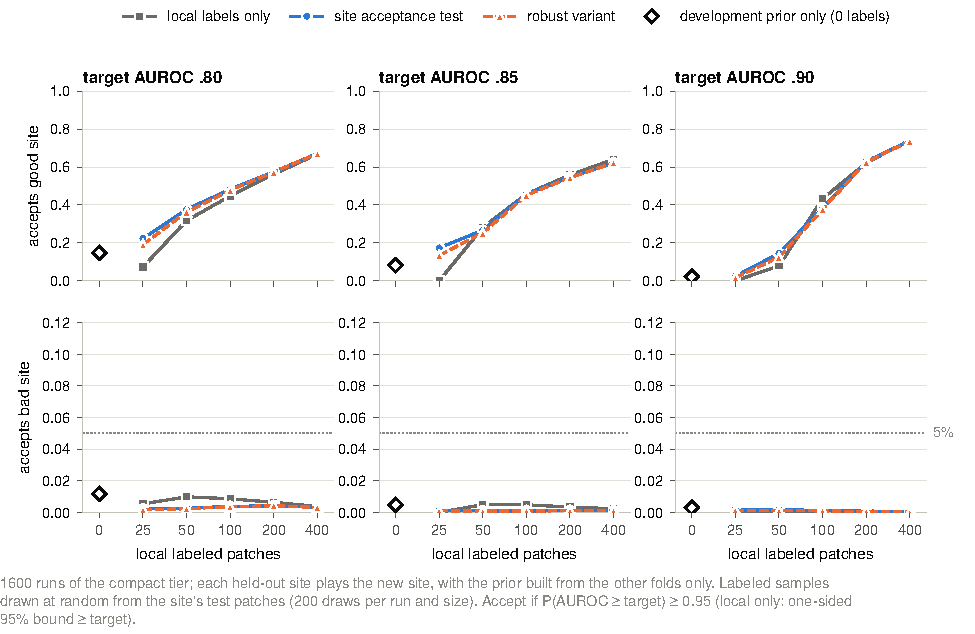
\includegraphics[width=\linewidth]{fig_sat_C}
  \caption{Validation of the site acceptance test at the compact tier, as in
  Fig.~\ref{M-fig:sat}.}
  \label{fig:sat-C}
\end{figure}

\begin{table}[width=\linewidth,pos=tbp]
\caption{Site acceptance test at the compact tier (1,600 runs), as in
Table~\ref{M-tab:sat}.}
\label{tab:sat-C}
\footnotesize
\setlength{\tabcolsep}{3pt}
% generated by src/v2/site_acceptance.py tables (results/v2/site_acceptance/sat_rows_*.csv)
\begin{tabular*}{\tblwidth}{@{\extracolsep{\fill}}lrrrrrrrrr@{}}
\toprule
 & & \multicolumn{2}{c}{$T=0.80$} & \multicolumn{2}{c}{$T=0.85$} & \multicolumn{2}{c}{$T=0.90$} & & \\
\cmidrule(lr){3-4}\cmidrule(lr){5-6}\cmidrule(lr){7-8}
Rule & $m$ & FA (\%) & power (\%) & FA (\%) & power (\%) & FA (\%) & power (\%) & MAE & cover. (\%) \\
\midrule
Development prior only & 0 & 1.2 & 15 & 0.5 & 8 & 0.3 & 2 & -- & -- \\
\addlinespace[2pt]
Site acceptance test & 25 & 0.2 & 22 & 0.1 & 17 & 0.2 & 2 & 0.042 & 90 \\
 & 50 & 0.3 & 38 & 0.1 & 27 & 0.2 & 14 & 0.035 & 90 \\
 & 100 & 0.4 & 48 & 0.1 & 46 & 0.1 & 38 & 0.027 & 90 \\
 & 200 & 0.4 & 57 & 0.1 & 55 & 0.1 & 63 & 0.021 & 91 \\
 & 400 & 0.3 & 67 & 0.1 & 62 & 0.0 & 74 & 0.015 & 92 \\
\addlinespace[2pt]
Local labels only & 25 & 0.5 & 7 & 0.0 & 0 & 0.0 & 0 & 0.068 & 94 \\
 & 50 & 1.0 & 32 & 0.5 & 28 & 0.1 & 8 & 0.047 & 92 \\
 & 100 & 0.9 & 45 & 0.5 & 46 & 0.1 & 43 & 0.033 & 92 \\
 & 200 & 0.6 & 56 & 0.3 & 56 & 0.1 & 62 & 0.022 & 92 \\
 & 400 & 0.4 & 67 & 0.2 & 64 & 0.0 & 74 & 0.015 & 93 \\
\bottomrule
\end{tabular*}

\end{table}

\begin{table}[width=\linewidth,pos=tbp]
\caption{Robust variant ($\epsilon=0.1$) at the standard tier (top) and the
compact tier (bottom), as in Table~\ref{M-tab:sat}. The variant was added after
the first validation and is therefore not independently validated.}
\label{tab:sat-robust}
\footnotesize
\setlength{\tabcolsep}{3pt}
% generated by src/v2/site_acceptance.py tables (results/v2/site_acceptance/sat_rows_*.csv)
\begin{tabular*}{\tblwidth}{@{\extracolsep{\fill}}lrrrrrrrrr@{}}
\toprule
 & & \multicolumn{2}{c}{$T=0.80$} & \multicolumn{2}{c}{$T=0.85$} & \multicolumn{2}{c}{$T=0.90$} & & \\
\cmidrule(lr){3-4}\cmidrule(lr){5-6}\cmidrule(lr){7-8}
Rule & $m$ & FA (\%) & power (\%) & FA (\%) & power (\%) & FA (\%) & power (\%) & MAE & cover. (\%) \\
\midrule
Robust variant & 25 & 1.4 & 58 & 0.6 & 28 & 0.2 & 14 & 0.029 & 93 \\
 & 50 & 1.7 & 72 & 0.8 & 47 & 0.3 & 27 & 0.024 & 92 \\
 & 100 & 1.2 & 83 & 0.7 & 62 & 0.2 & 43 & 0.019 & 92 \\
 & 200 & 0.8 & 89 & 0.6 & 71 & 0.2 & 51 & 0.015 & 92 \\
 & 400 & 0.4 & 93 & 0.3 & 79 & 0.1 & 60 & 0.011 & 93 \\
\bottomrule
\end{tabular*}
\\[6pt]
% generated by src/v2/site_acceptance.py tables (results/v2/site_acceptance/sat_rows_*.csv)
\begin{tabular*}{\tblwidth}{@{\extracolsep{\fill}}lrrrrrrrrr@{}}
\toprule
 & & \multicolumn{2}{c}{$T=0.80$} & \multicolumn{2}{c}{$T=0.85$} & \multicolumn{2}{c}{$T=0.90$} & & \\
\cmidrule(lr){3-4}\cmidrule(lr){5-6}\cmidrule(lr){7-8}
Rule & $m$ & FA (\%) & power (\%) & FA (\%) & power (\%) & FA (\%) & power (\%) & MAE & cover. (\%) \\
\midrule
Robust variant & 25 & 0.2 & 19 & 0.1 & 13 & 0.1 & 2 & 0.043 & 91 \\
 & 50 & 0.2 & 36 & 0.1 & 25 & 0.1 & 12 & 0.035 & 91 \\
 & 100 & 0.4 & 48 & 0.1 & 45 & 0.1 & 38 & 0.027 & 91 \\
 & 200 & 0.4 & 57 & 0.1 & 54 & 0.1 & 63 & 0.021 & 91 \\
 & 400 & 0.3 & 67 & 0.1 & 62 & 0.0 & 74 & 0.015 & 92 \\
\bottomrule
\end{tabular*}

\end{table}

\begin{table}[width=\linewidth,pos=tbp]
\caption{False acceptance (\%) / power (\%) by cohort at a target of 0.85, with
50 and 100 local labels, for the site acceptance test, its robust variant and
local labels alone. Bad: number of runs whose true site AUROC is below 0.85.}
\label{tab:sat-cohorts}
\footnotesize
\setlength{\tabcolsep}{3pt}
% generated by src/v2/site_acceptance.py tables; cells: false acceptance (%) / power (%), T = 0.85
\begin{tabular*}{\tblwidth}{@{\extracolsep{\fill}}llrrrrrrr@{}}
\toprule
Tier & Cohort & bad & Site 50 & Site 100 & Robust 50 & Robust 100 & Local 50 & Local 100 \\
\midrule
S & Camelyon17 & 14 & 2.5 / 87 & 0.9 / 95 & 1.9 / 81 & 0.7 / 93 & 0.3 / 60 & 0.2 / 88 \\
 & Canine cSCC & 99 & 1.5 / 27 & 1.2 / 45 & 1.4 / 26 & 1.1 / 44 & 0.9 / 26 & 0.7 / 45 \\
 & MIDOG 2021 & 62 & 0.0 / 5 & 0.2 / 14 & 0.0 / 4 & 0.2 / 13 & 0.4 / 4 & 0.7 / 11 \\
 & MIDOG++ & 73 & 0.7 / 50 & 0.6 / 65 & 0.6 / 46 & 0.5 / 63 & 0.3 / 15 & 0.3 / 34 \\
\addlinespace[3pt]
C & Camelyon17 & 114 & 0.8 / 49 & 0.7 / 80 & 0.7 / 46 & 0.6 / 79 & 0.4 / 49 & 0.4 / 76 \\
 & Canine cSCC & 376 & 0.0 / 0 & 0.0 / 0 & 0.0 / 0 & 0.0 / 0 & 0.4 / 5 & 0.3 / 8 \\
 & MIDOG 2021 & 173 & 0.0 / 3 & 0.0 / 10 & 0.0 / 2 & 0.0 / 9 & 0.3 / 3 & 0.3 / 9 \\
 & MIDOG++ & 387 & 0.0 / 3 & 0.0 / 9 & 0.0 / 2 & 0.0 / 9 & 0.7 / 6 & 0.7 / 15 \\
\bottomrule
\end{tabular*}

\end{table}

\clearpage
%% Appendix: supplementary results (MedIA revision, v2 pipeline).
%% Figures: paper/media/figs (rendered from snapshot 1381bdd759f9 by src/v2/make_figures_v2.py --freeze).
%% Tables: paper/media/tables (src/v2/paper_tables.py). Ladder-only rank agreement:
%% results/v2/analysis/S_ladder_only/cross/kendall_id.csv.
\section{Compact-tier results}
\label{app:compact}

This section gives the compact-tier counterparts of the main-text figures
and tables. Table~\ref{tab:main-C} lists worst-domain and mean AUROC,
Fig.~\ref{fig:perdomain-C} the per-domain results, Fig.~\ref{fig:variance-C}
the variance decomposition, Fig.~\ref{fig:power-C} the power curves and
Fig.~\ref{fig:ranks-C} the rankings. Figure~\ref{fig:seedspread} shows the
individual seeds of three compact-tier arms next to the best standard-tier arm.

\begin{table}[width=\linewidth,pos=p]
\caption{Compact tier: worst-domain AUROC (rank among the 20 arms) and mean
AUROC over held-out domains, ID-validation selection, five seeds. Bold: best
worst-domain AUROC in the cohort. $^{\dagger}$Transductive.}
\label{tab:main-C}
\footnotesize
\setlength{\tabcolsep}{3pt}
% generated by src/v2/paper_tables.py from results/v2/analysis/C/*/summary_id.csv, ranks_id.csv
\begin{tabular*}{\tblwidth}{@{\extracolsep{\fill}}l*{4}{rr}@{}}
\toprule
Arm & \multicolumn{2}{c}{Camelyon17 ($K=5$)} & \multicolumn{2}{c}{Canine cSCC ($K=5$)} & \multicolumn{2}{c}{MIDOG 2021 ($K=3$)} & \multicolumn{2}{c}{MIDOG++ ($K=7$)} \\
\cmidrule(lr){2-3}\cmidrule(lr){4-5}\cmidrule(lr){6-7}\cmidrule(lr){8-9}
 & worst (rank) & mean & worst (rank) & mean & worst (rank) & mean & worst (rank) & mean \\
\midrule
\multicolumn{9}{@{}l}{\emph{Reference and controls}}\\
ERM & 0.698 (13) & 0.844 & 0.551 (18) & 0.714 & 0.765 (17) & 0.801 & 0.766 (13) & 0.827 \\
Compute-matched ERM & 0.727 (12) & 0.848 & 0.466 (20) & 0.693 & 0.789 (13) & 0.818 & \textbf{0.862} (1) & 0.887 \\
\addlinespace[2pt]
\multicolumn{9}{@{}l}{\emph{Domain-aware training}}\\
GroupDRO & 0.670 (14) & 0.830 & 0.579 (17) & 0.715 & 0.764 (18) & 0.802 & 0.731 (16) & 0.804 \\
IRM & 0.607 (19) & 0.828 & 0.589 (16) & 0.718 & 0.785 (14) & 0.809 & 0.741 (15) & 0.805 \\
CORAL & 0.637 (17) & 0.816 & 0.596 (15) & 0.723 & 0.803 (10) & 0.808 & 0.802 (9) & 0.845 \\
MixStyle & 0.665 (15) & 0.849 & 0.605 (13) & 0.735 & 0.777 (15) & 0.794 & 0.709 (17) & 0.794 \\
Fish & 0.615 (18) & 0.842 & 0.502 (19) & 0.676 & 0.676 (20) & 0.759 & 0.667 (20) & 0.765 \\
LISA & 0.735 (11) & 0.846 & 0.669 (10) & 0.718 & 0.714 (19) & 0.762 & 0.691 (18) & 0.778 \\
\addlinespace[2pt]
\multicolumn{9}{@{}l}{\emph{Stain normalization and color}}\\
Macenko$^{\dagger}$ & 0.904 (4) & 0.943 & 0.698 (7) & 0.813 & 0.870 (2) & 0.878 & 0.828 (2) & 0.868 \\
Macenko (per tile) & 0.524 (20) & 0.861 & 0.671 (9) & 0.763 & 0.844 (7) & 0.861 & 0.816 (3) & 0.849 \\
H\&E jitter & 0.904 (3) & 0.933 & 0.674 (8) & 0.795 & 0.864 (5) & 0.876 & 0.809 (8) & 0.843 \\
TIA-style$^{\dagger}$ & 0.889 (6) & 0.951 & 0.730 (6) & 0.777 & 0.864 (6) & 0.879 & 0.810 (7) & 0.853 \\
Aug-only control & 0.815 (10) & 0.921 & 0.745 (5) & 0.766 & 0.805 (9) & 0.819 & 0.670 (19) & 0.745 \\
\addlinespace[2pt]
\multicolumn{9}{@{}l}{\emph{Self-supervision}}\\
SimCLR & 0.897 (5) & 0.939 & 0.613 (12) & 0.734 & 0.795 (12) & 0.806 & 0.789 (10) & 0.838 \\
SimCLR+SAM & \textbf{0.909} (1) & 0.944 & 0.603 (14) & 0.738 & 0.797 (11) & 0.801 & 0.781 (12) & 0.830 \\
\addlinespace[2pt]
\multicolumn{9}{@{}l}{\emph{Sharpness-aware}}\\
SAM & 0.639 (16) & 0.825 & 0.614 (11) & 0.725 & 0.776 (16) & 0.809 & 0.757 (14) & 0.815 \\
\addlinespace[2pt]
\multicolumn{9}{@{}l}{\emph{Test-time adaptation}}\\
BN-adapt (ERM)$^{\dagger}$ & 0.854 (9) & 0.920 & 0.801 (2) & 0.836 & 0.865 (3) & 0.880 & 0.814 (4) & 0.834 \\
TENT (ERM)$^{\dagger}$ & 0.874 (7) & 0.933 & 0.799 (3) & 0.835 & 0.865 (4) & 0.878 & 0.814 (5) & 0.830 \\
BN-adapt (SimCLR)$^{\dagger}$ & 0.858 (8) & 0.938 & \textbf{0.822} (1) & 0.836 & 0.842 (8) & 0.852 & 0.786 (11) & 0.830 \\
BN-adapt (H\&E jitter)$^{\dagger}$ & 0.908 (2) & 0.950 & 0.798 (4) & 0.831 & \textbf{0.877} (1) & 0.891 & 0.812 (6) & 0.845 \\
\bottomrule
\end{tabular*}

\end{table}

\begin{figure}[pos=p]
  \centering
  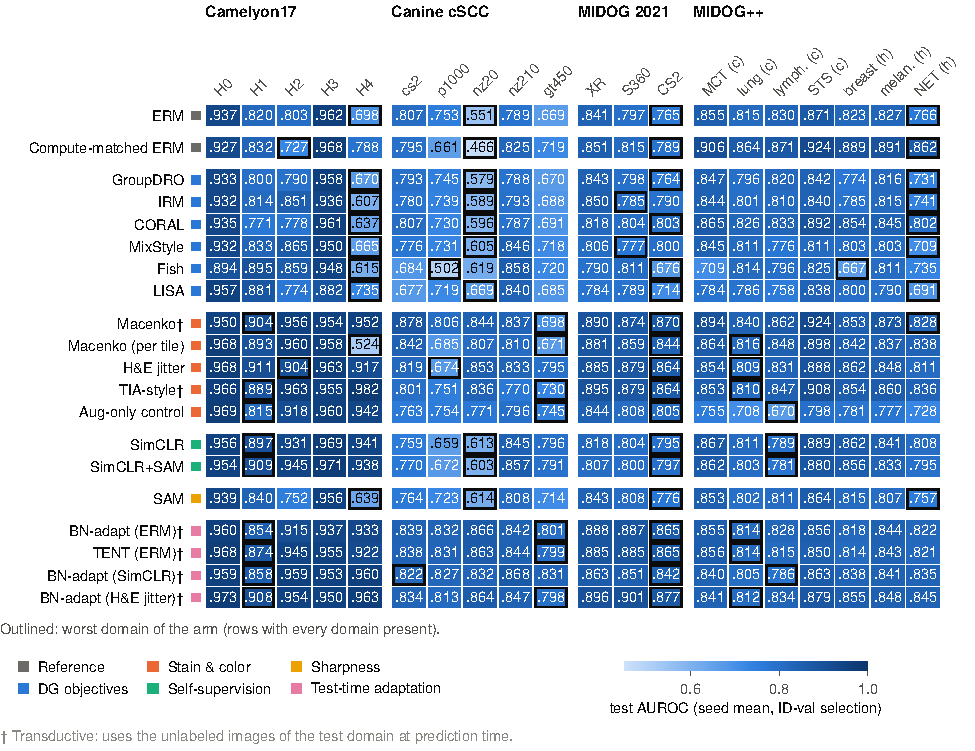
\includegraphics[width=\linewidth]{fig_perdomain_C}
  \caption{Test AUROC of every compact-tier arm at every held-out domain (mean
  over five seeds; ID-validation selection). Outlined: each arm's worst domain.
  $^{\dagger}$Transductive.}
  \label{fig:perdomain-C}
\end{figure}

\begin{figure}[pos=p]
  \centering
  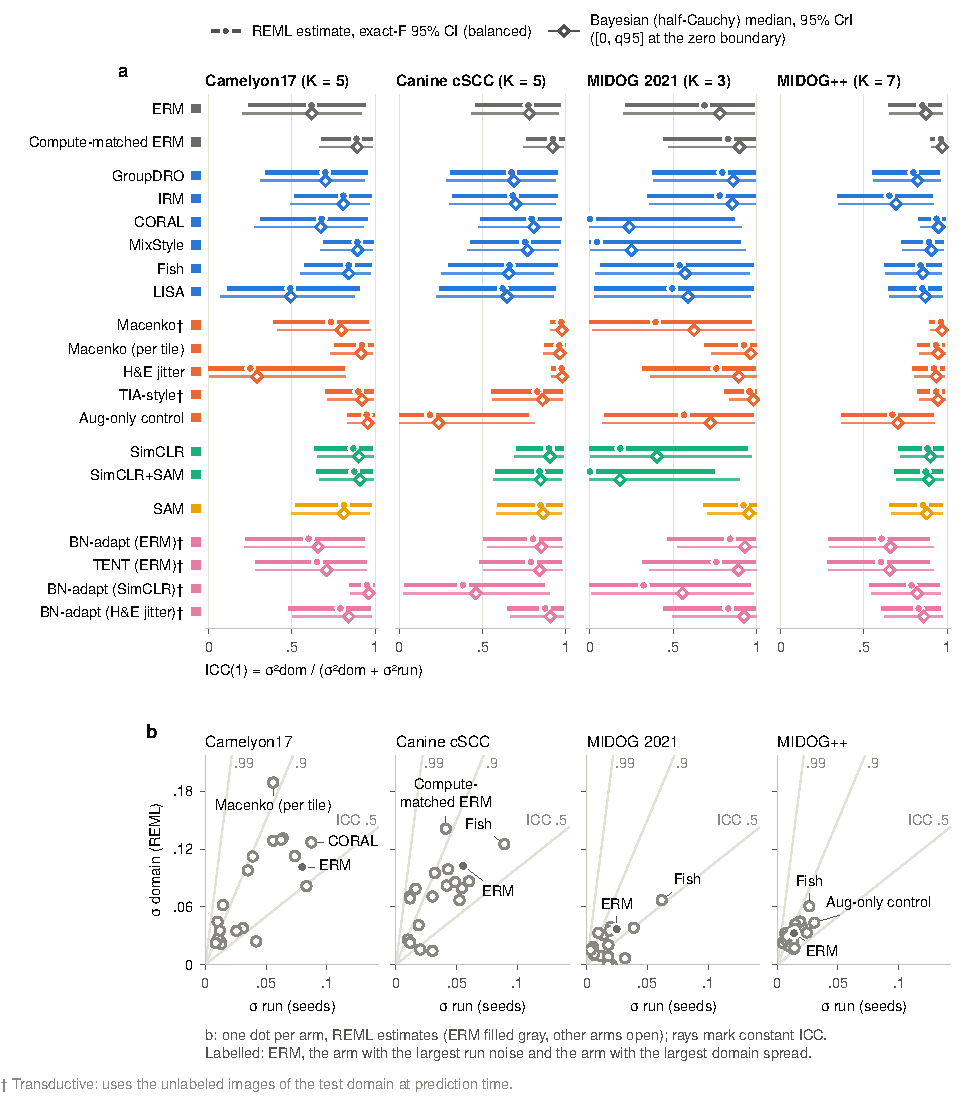
\includegraphics[width=0.92\linewidth]{fig_variance_C}
  \caption{Variance decomposition at the compact tier, as in
  Fig.~\ref{M-fig:variance}. $^{\dagger}$Transductive.}
  \label{fig:variance-C}
\end{figure}

\begin{figure}[pos=tbp]
  \centering
  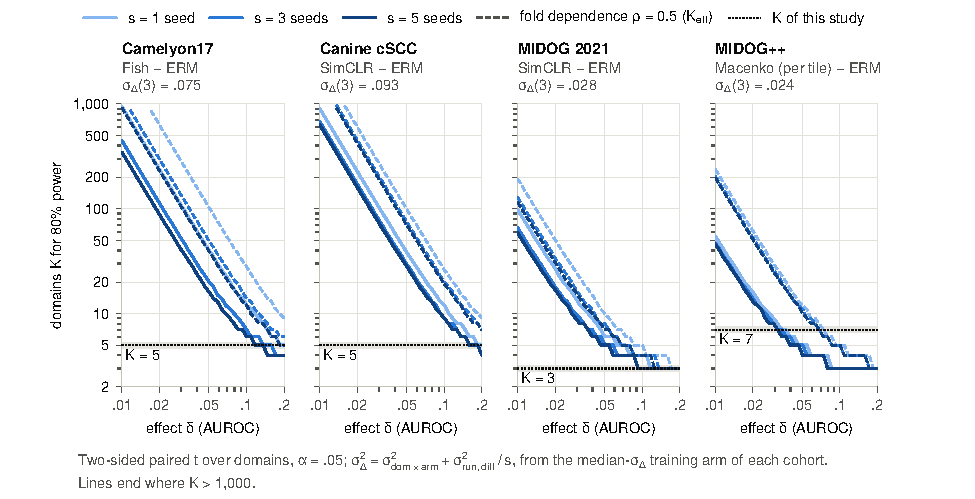
\includegraphics[width=\linewidth]{fig_power_C}
  \caption{Domains needed for 80\% power at the compact tier, as in
  Fig.~\ref{M-fig:power}.}
  \label{fig:power-C}
\end{figure}

\begin{figure}[pos=p]
  \centering
  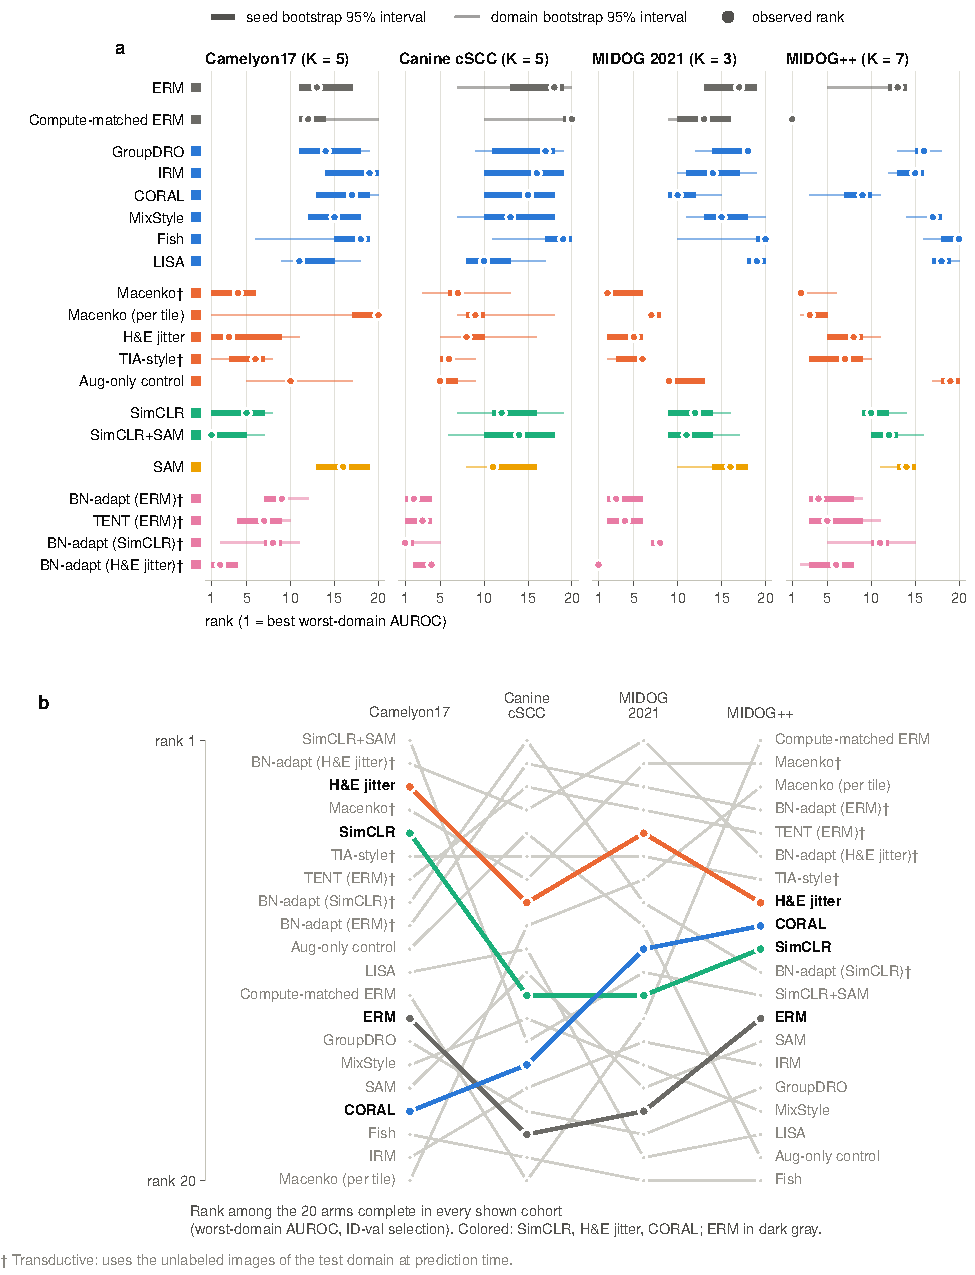
\includegraphics[width=0.85\linewidth]{fig_ranks_C}
  \caption{Rankings at the compact tier, as in Fig.~\ref{M-fig:ranks}.
  $^{\dagger}$Transductive.}
  \label{fig:ranks-C}
\end{figure}

\begin{figure}[pos=tbp]
  \centering
  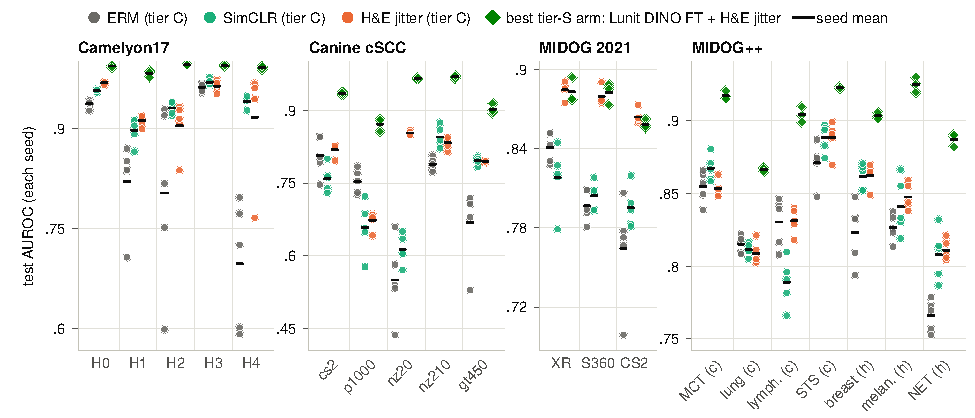
\includegraphics[width=\linewidth]{fig_seedspread}
  \caption{Individual seeds at every held-out domain for compact-tier ERM,
  SimCLR and H\&E jitter, and for the best standard-tier arm (fine-tuned Lunit
  DINO with H\&E jitter, the arm with the highest mean worst-domain AUROC over
  the four cohorts, 0.895). Bars mark seed means. The $y$-axes are scaled per
  cohort.}
  \label{fig:seedspread}
\end{figure}

\clearpage
\section{Model-selection rules}
\label{app:selection}

Figures~\ref{fig:selection-S} and \ref{fig:selection-C} show each arm's mean
difference from ERM under the four selection rules. All rules use the same
ten checkpoints of the same runs (Section~\ref{M-sec:protocol-lodo}), so the
differences come from selection alone. The $\tau_b$ values printed in the
figures compare the rankings of these mean differences; those of
Table~\ref{M-tab:selection} compare worst-domain rankings. At the standard tier
the rules agree closely. At the compact tier the OOD-validation and oracle
rules reorder the canine and Camelyon17 arms considerably.

\begin{figure}[pos=p]
  \centering
  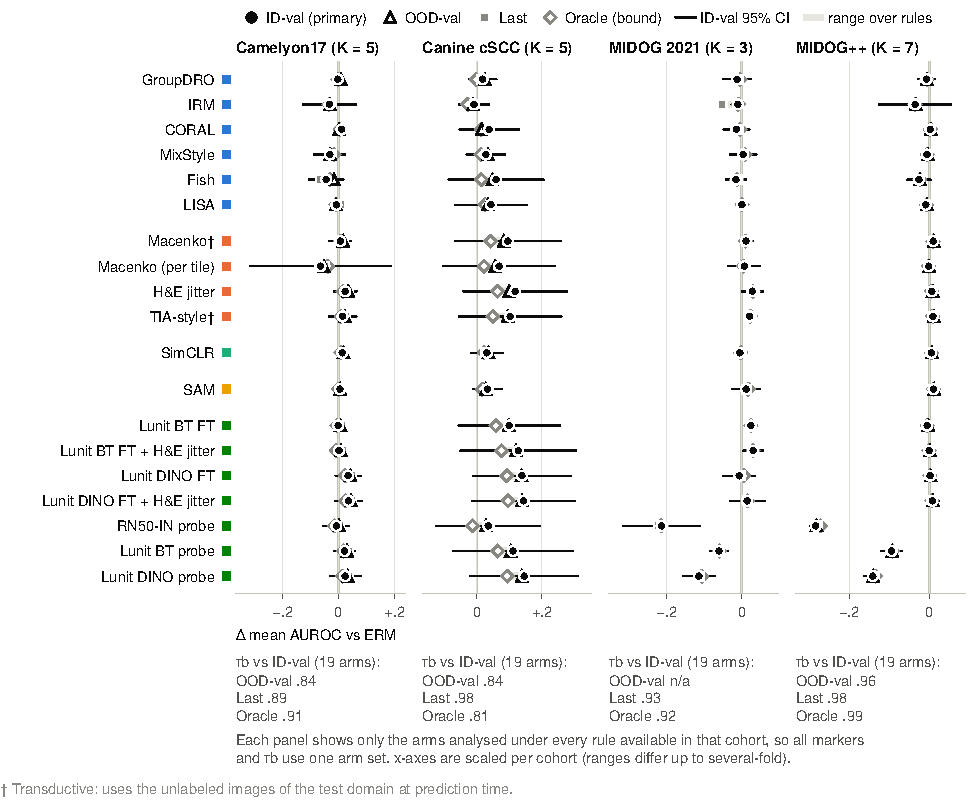
\includegraphics[width=\linewidth]{fig_selection_S}
  \caption{Standard tier: mean AUROC difference from ERM under ID-validation
  (primary, with 95\% interval), OOD-validation, last-checkpoint and oracle
  selection. Each panel shows the arms analyzed under every rule available in
  the cohort. $^{\dagger}$Transductive.}
  \label{fig:selection-S}
\end{figure}

\begin{figure}[pos=p]
  \centering
  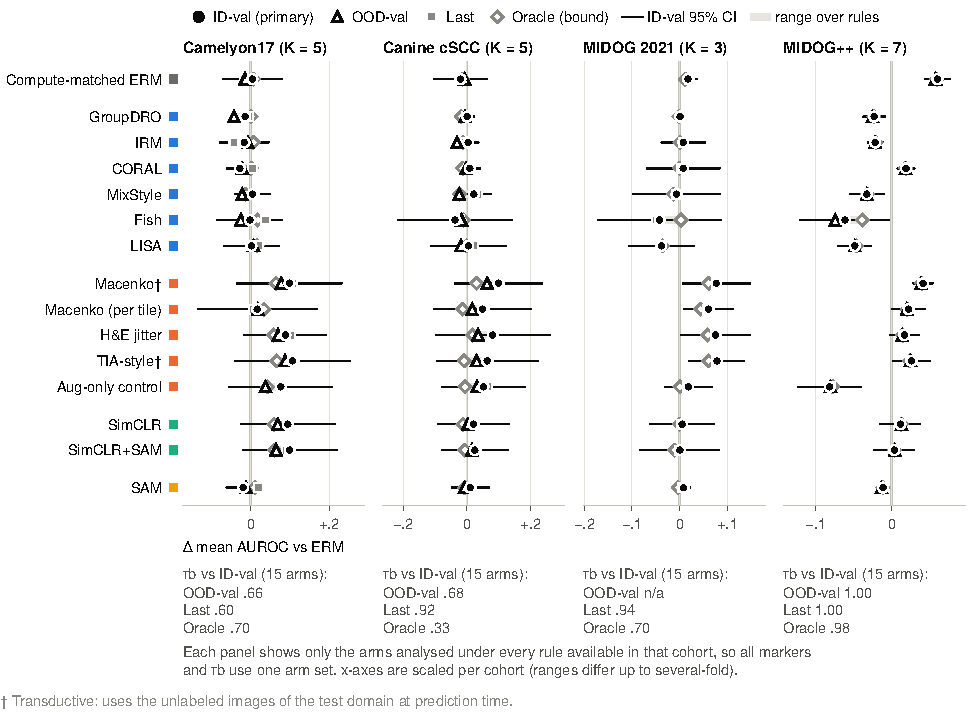
\includegraphics[width=\linewidth]{fig_selection_C}
  \caption{Compact tier: mean AUROC difference from ERM under the four
  selection rules, as in Fig.~\ref{fig:selection-S}.
  $^{\dagger}$Transductive.}
  \label{fig:selection-C}
\end{figure}

\clearpage
\section{Calibration}
\label{app:calibration}

Figures~\ref{fig:calibration-S} and \ref{fig:calibration-C} give the expected
calibration error (Eq.~\ref{M-eq:ece}) of every arm, averaged over domains and at
its worst domain, and reliability diagrams for the fold in which ERM performs
worst. At the standard tier, one of the two fine-tuned foundation models with
H\&E jitter is the best calibrated arm on every cohort. ERM is poorly calibrated on the
canine cohort and MIDOG~2021 (mean ECE 0.180 on both). Calibration varies
between domains as much as discrimination does: for most arms the worst-domain
ECE is well above the mean.

\begin{figure}[pos=p]
  \centering
  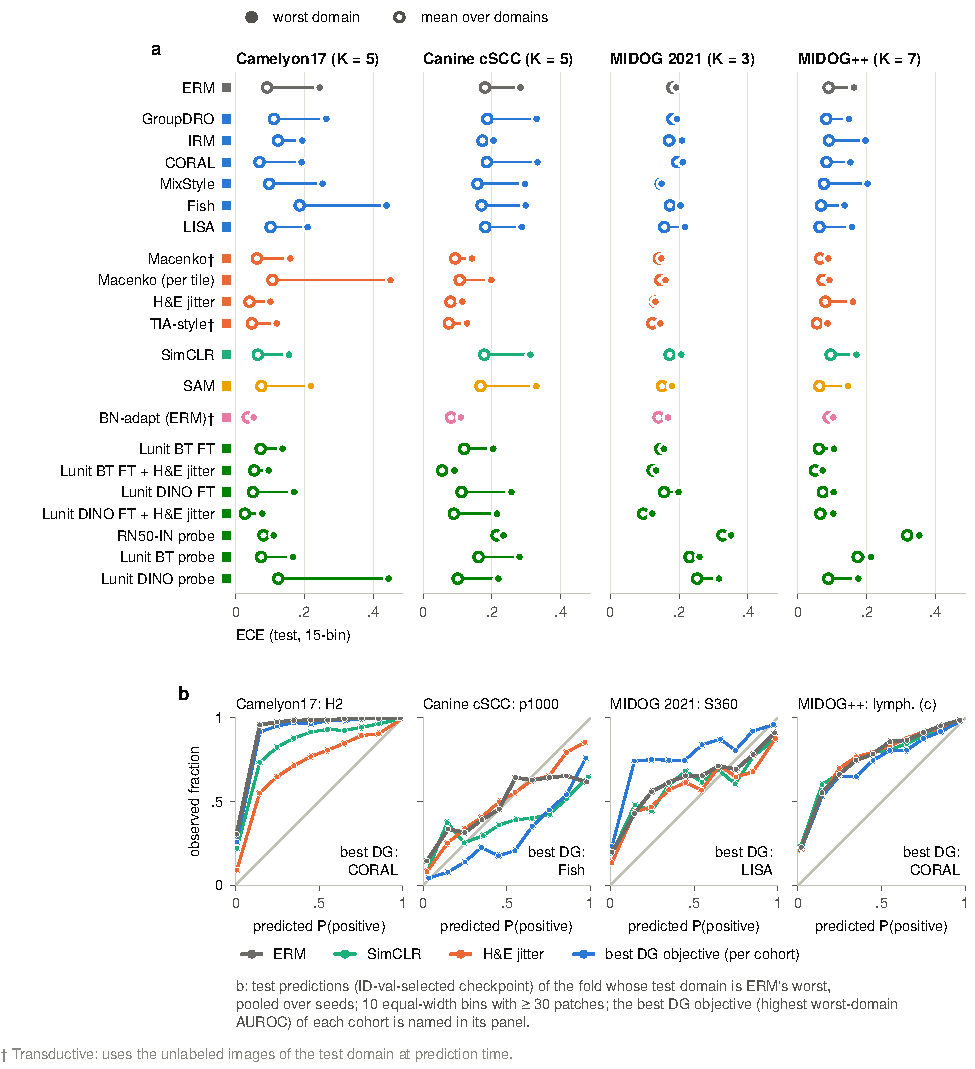
\includegraphics[width=0.92\linewidth]{fig_calibration_S}
  \caption{Calibration at the standard tier. (a) Test ECE (15 equal-width bins)
  at the worst domain (filled) and averaged over domains (open). (b) Reliability
  diagrams for the fold whose test domain is ERM's worst, pooled over seeds.
  $^{\dagger}$Transductive.}
  \label{fig:calibration-S}
\end{figure}

\begin{figure}[pos=p]
  \centering
  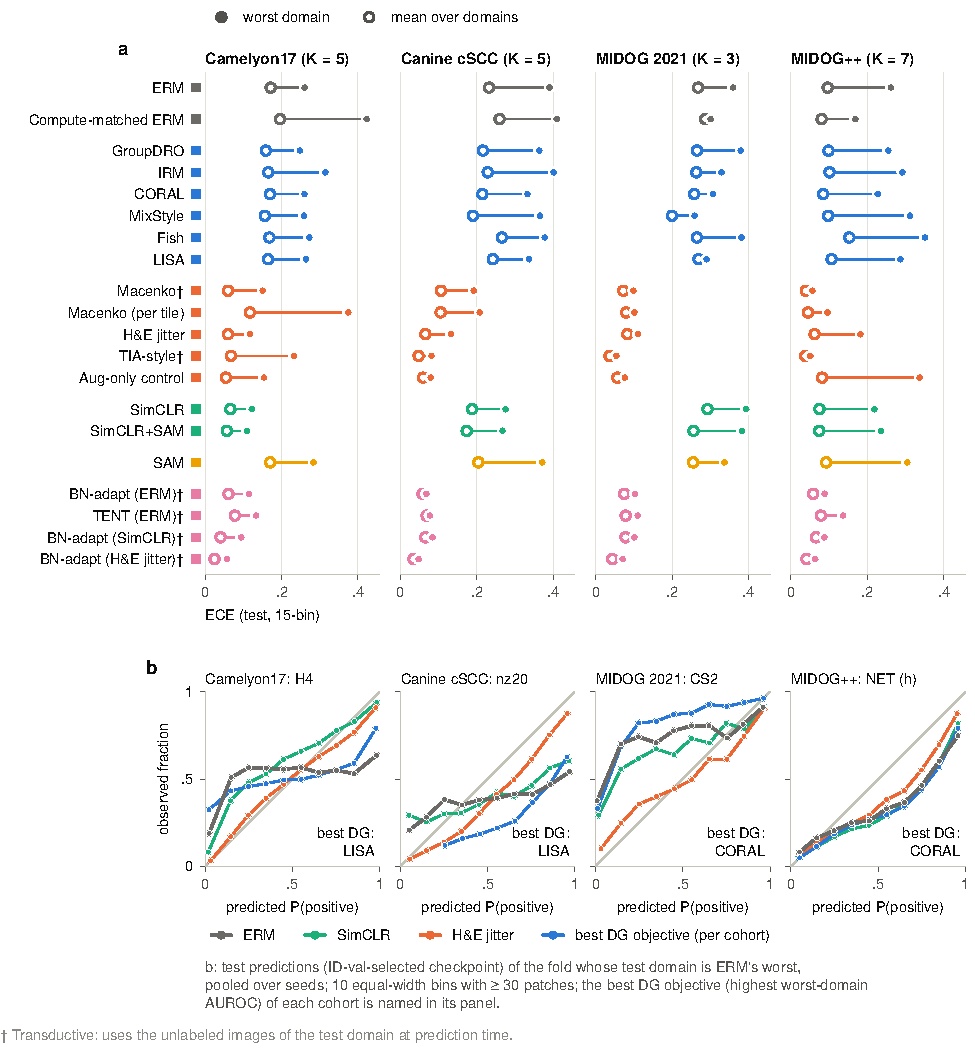
\includegraphics[width=0.92\linewidth]{fig_calibration_C}
  \caption{Calibration at the compact tier, as in Fig.~\ref{fig:calibration-S}.
  $^{\dagger}$Transductive.}
  \label{fig:calibration-C}
\end{figure}

\clearpage
\section{Representation ladder}
\label{app:ladder}

Figure~\ref{fig:ladder} compares nine frozen backbones under one linear-probe
protocol: four ImageNet-1k models (ResNet-18, ResNet-50, ConvNeXt-T
\citep{liu2022convnext}, ViT-B/16), a ViT-B/16 pre-trained with weak supervision on
3.6 billion images and fine-tuned on ImageNet-1k \citep{singh2022swag}, and four Lunit pathology models
\citep{kang2023benchmarking}. The Lunit Barlow Twins ResNet-50 and DINO ViT-S/16
are the best frozen encoders on the canine cohort and, by mean AUROC, on
Camelyon17; by worst-domain AUROC on Camelyon17 the DINO ViT is fourth, behind
Barlow Twins and two ImageNet models. On the mitosis cohorts every
frozen probe is well below fine-tuned ERM, and the Lunit SwAV ResNet-50 is
below the ImageNet ResNet-50 averaged over the four cohorts. Within this
probe-only ladder, the two mitosis cohorts rank the backbones almost
identically ($\tau_b=0.83$), while the two tumor cohorts barely agree
($\tau_b=0.17$).

\begin{figure}[pos=tbp]
  \centering
  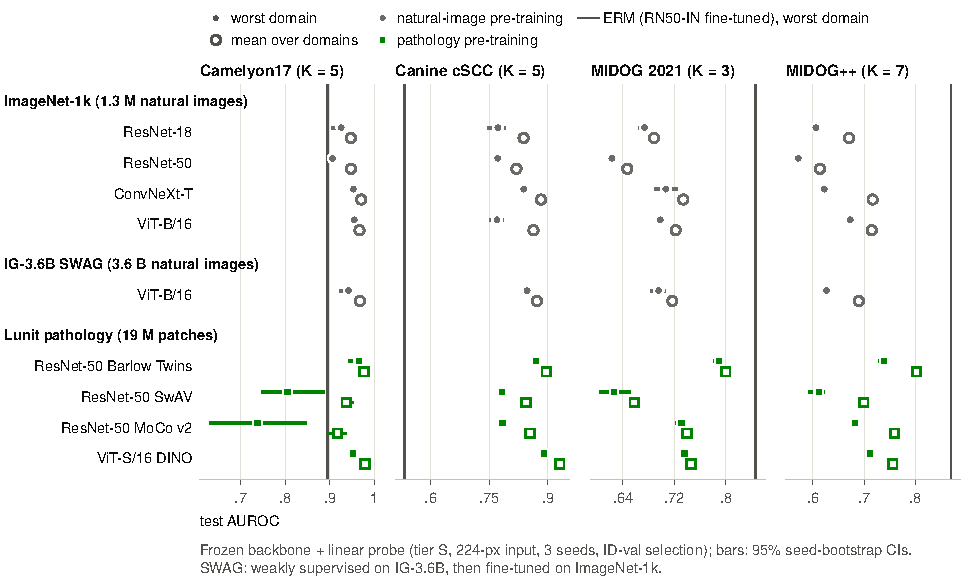
\includegraphics[width=\linewidth]{fig_ladder}
  \caption{Frozen backbones with a linear probe (standard tier, 224~px input,
  three seeds, ID-validation selection): worst-domain (filled, with
  seed-bootstrap 95\% interval) and mean AUROC (open). Vertical line: fine-tuned
  ImageNet ResNet-50 ERM, worst domain.}
  \label{fig:ladder}
\end{figure}

\clearpage
\section{Sensitivity analyses}
\label{app:sensitivity}

\paragraph{Scale normalization of MIDOG~2021} Figure~\ref{fig:sensitivity}
compares the compact-tier results on the scale-normalized (primary) and the
un-normalized MIDOG~2021 cohort.

\begin{figure}[pos=tbp]
  \centering
  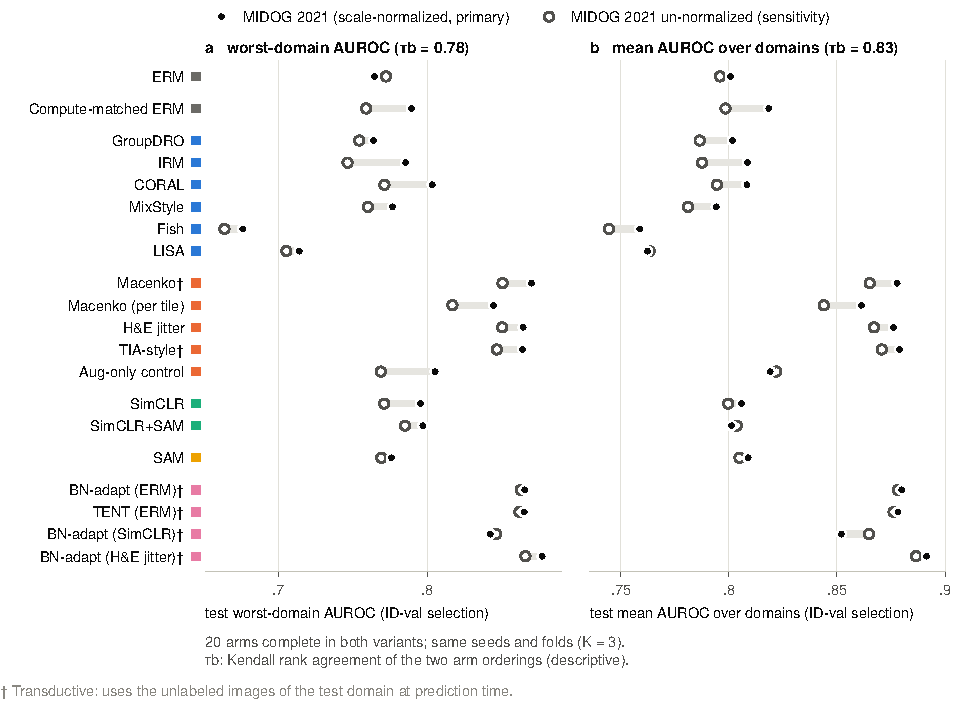
\includegraphics[width=0.9\linewidth]{fig_sensitivity_C}
  \caption{MIDOG~2021 with and without scale normalization (compact tier,
  20 arms, same seeds and folds): (a) worst-domain and (b) mean AUROC.
  $^{\dagger}$Transductive.}
  \label{fig:sensitivity}
\end{figure}

\paragraph{PatchCamelyon} Table~\ref{tab:pcam} gives the PatchCamelyon test
AUROC of the Camelyon17 models at the ID-validation-selected checkpoint,
averaged over seeds, with its mean and minimum over the five Camelyon17 folds.
The score is never used for selection. Test-time adaptation is not evaluated
on PatchCamelyon.

\begin{table}[width=\linewidth,pos=t]
\caption{PatchCamelyon test AUROC of the Camelyon17 models: mean and minimum
over the five folds of the seed-mean AUROC. $^{\dagger}$Transductive.}
\label{tab:pcam}
\footnotesize
% generated by src/v2/paper_tables.py from the pcam field of the frozen run records (ID-val checkpoint)
\begin{tabular*}{\tblwidth}{@{\extracolsep{\fill}}lrrrr@{}}
\toprule
 & \multicolumn{2}{c}{Compact tier} & \multicolumn{2}{c}{Standard tier} \\
\cmidrule(lr){2-3}\cmidrule(lr){4-5}
Arm & mean & min over folds & mean & min over folds \\
\midrule
ERM & 0.698 & 0.641 & 0.772 & 0.665 \\
Compute-matched ERM & 0.652 & 0.542 & -- & -- \\
GroupDRO & 0.697 & 0.634 & 0.791 & 0.738 \\
IRM & 0.716 & 0.675 & 0.753 & 0.669 \\
CORAL & 0.691 & 0.621 & 0.772 & 0.707 \\
MixStyle & 0.739 & 0.703 & 0.780 & 0.702 \\
Fish & 0.647 & 0.581 & 0.729 & 0.618 \\
LISA & 0.672 & 0.576 & 0.756 & 0.631 \\
Macenko$^{\dagger}$ & 0.765 & 0.677 & 0.752 & 0.634 \\
Macenko (per tile) & 0.756 & 0.686 & 0.837 & 0.784 \\
H\&E jitter & 0.768 & 0.664 & 0.843 & 0.801 \\
TIA-style$^{\dagger}$ & 0.802 & 0.730 & 0.858 & 0.838 \\
Aug-only control & 0.777 & 0.725 & -- & -- \\
SimCLR & 0.743 & 0.701 & 0.753 & 0.656 \\
SimCLR+SAM & 0.761 & 0.724 & -- & -- \\
SAM & 0.690 & 0.544 & 0.780 & 0.684 \\
Lunit BT FT & -- & -- & 0.838 & 0.791 \\
Lunit BT FT + H\&E jitter & -- & -- & 0.850 & 0.781 \\
Lunit DINO FT & -- & -- & 0.905 & 0.874 \\
Lunit DINO FT + H\&E jitter & -- & -- & 0.908 & 0.895 \\
RN50-IN probe & -- & -- & 0.820 & 0.806 \\
Lunit BT probe & -- & -- & 0.889 & 0.866 \\
Lunit DINO probe & -- & -- & 0.886 & 0.867 \\
\bottomrule
\end{tabular*}

\end{table}

\paragraph{Hyperparameters} Figures~\ref{fig:tuning-S} and \ref{fig:tuning-C}
show how test AUROC of the seed-0 tuning runs varies across each grid. Test
AUROC is shown only to display this sensitivity; selection used ID-validation
AUROC (Section~\ref{app:tuning}).

\begin{figure}[pos=p]
  \centering
  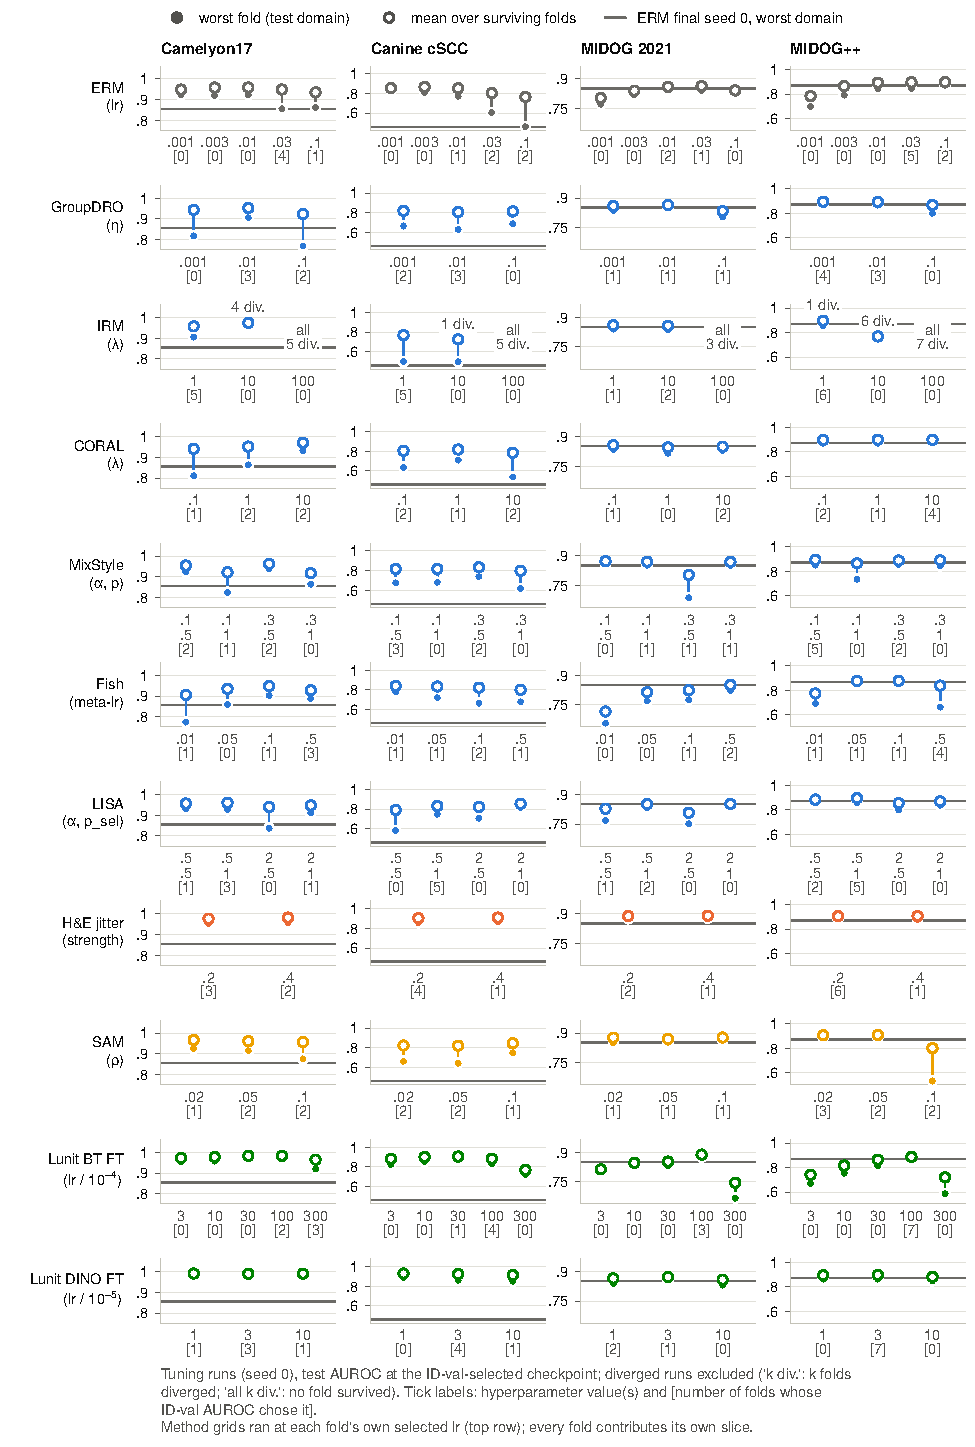
\includegraphics[width=0.78\linewidth]{fig_tuning_S}
  \caption{Standard-tier tuning runs (seed 0): test AUROC at the
  ID-validation-selected checkpoint for each grid value, worst fold (filled) and
  mean over folds (open). Brackets: number of folds whose ID-validation AUROC
  selected the value. `$k$ div.': $k$ folds diverged. Gray line: worst domain of
  final ERM, seed~0.}
  \label{fig:tuning-S}
\end{figure}

\begin{figure}[pos=p]
  \centering
  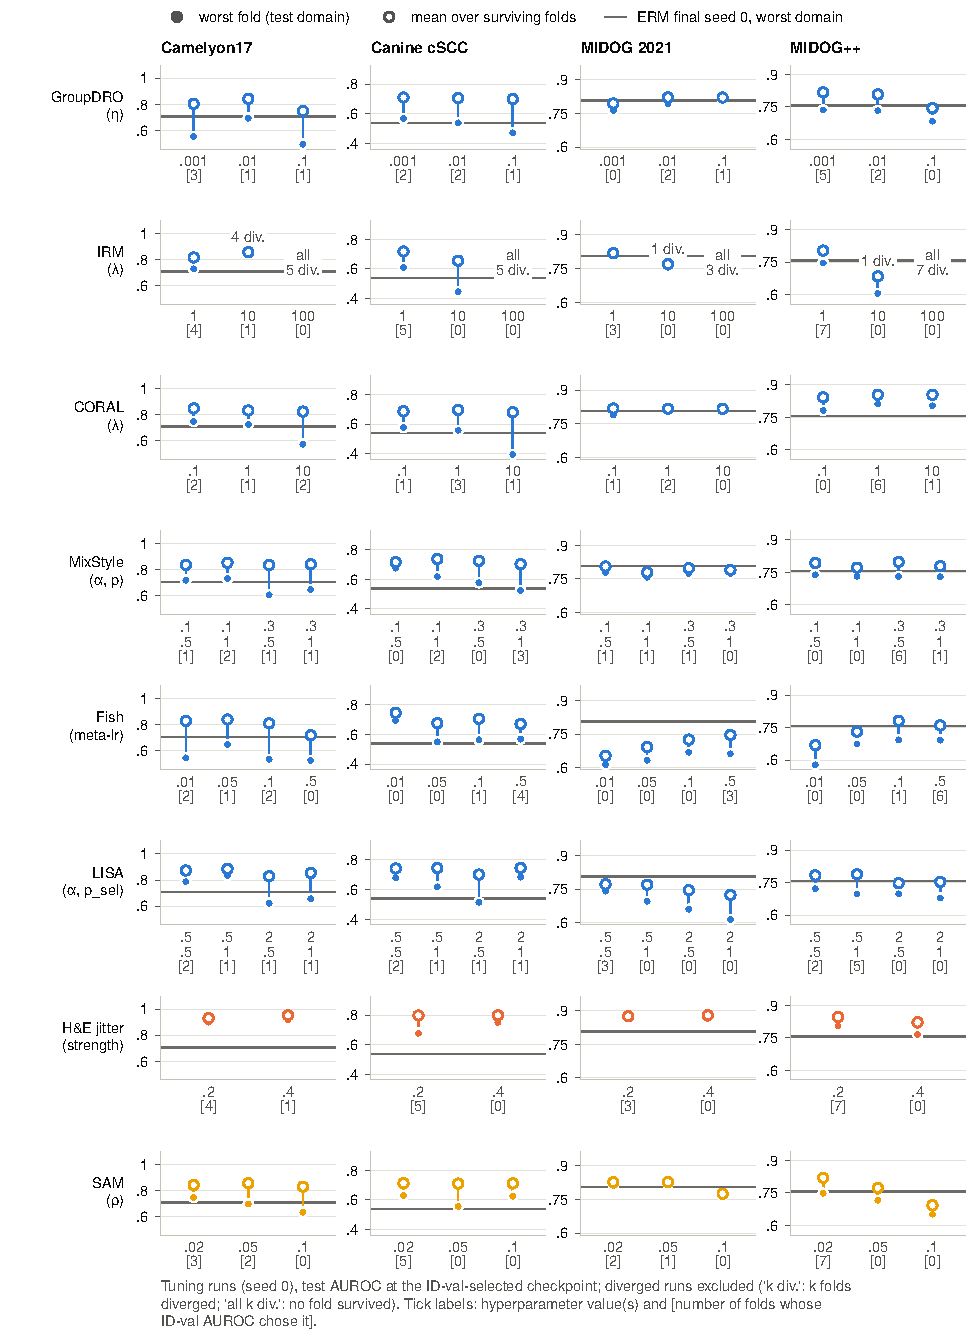
\includegraphics[width=0.78\linewidth]{fig_tuning_C}
  \caption{Compact-tier tuning runs (seed 0), as in Fig.~\ref{fig:tuning-S}.}
  \label{fig:tuning-C}
\end{figure}

\clearpage
\section{Response shape}
\label{app:response}

Table~\ref{tab:response} summarizes Oldham's correlation $r$ between each
arm's per-domain gain over ERM and the per-domain mean of the two
(Section~\ref{sec:protocol-response}). A negative $r$ means that the arm gains
most where both arms do worst, so it narrows the spread between domains. On the
tumor cohorts at both tiers and on MIDOG~2021 at the compact tier, most arms
have a negative $r$; on the canine cohort at the standard tier, all 20 do. The
Pitman--Morgan test is significant for 14 of them. The exact sign-flip test
cannot reach $p<0.05$ with five or fewer domains, and on MIDOG++ its smallest
$p$ is 0.078 at the standard tier. We therefore read the pattern as consistent but not established.

\begin{table}[width=\linewidth,pos=t]
\caption{Response shape: number of arms with negative Oldham's correlation $r$,
median $r$, number of arms with Pitman--Morgan $p<0.05$, and the smallest
exact sign-flip $p$ over arms.}
\label{tab:response}
\footnotesize
% generated by src/v2/paper_tables.py from response_id.csv
\begin{tabular*}{\tblwidth}{@{\extracolsep{\fill}}llrrrrr@{}}
\toprule
Tier & Cohort & $K$ & $r<0$ & median $r$ & Pitman--Morgan $p<0.05$ & smallest exact $p$ \\
\midrule
S & Camelyon17 & 5 & 15/20 & -0.36 & 7 & 0.062 \\
 & Canine cSCC & 5 & 20/20 & -0.91 & 14 & 0.062 \\
 & MIDOG 2021 & 3 & 10/20 & -0.01 & 0 & 0.250 \\
 & MIDOG++ & 7 & 4/20 & +0.13 & 5 & 0.078 \\
\addlinespace[3pt]
C & Camelyon17 & 5 & 12/19 & -0.52 & 7 & 0.125 \\
 & Canine cSCC & 5 & 17/19 & -0.73 & 6 & 0.062 \\
 & MIDOG 2021 & 3 & 16/19 & -0.94 & 6 & 0.250 \\
 & MIDOG++ & 7 & 10/19 & -0.03 & 0 & 0.281 \\
\bottomrule
\end{tabular*}

\end{table}

\clearpage
%% Appendix: hyperparameter tuning and diverged runs (MedIA revision, v2 pipeline).
%% Every number is computed from results/v2/tuning_results.csv (one row per seed-0
%% tuning record in $V2/runs_tune, 1,378 rows) and results/v2/selected_hparams.json,
%% both written by src/v2/select_hparams.py; divergence steps from the
%% `diverged_at_step` field of the records. Test AUROC of tuning runs is not reported.
\section{Hyperparameter tuning and diverged runs}
\label{app:tuning}

\paragraph{Protocol} Hyperparameters are tuned with seed~0 on the grids of
Table~\ref{M-tab:arms}, separately for every fold
(Section~\ref{M-sec:protocol-lodo}). Each fold keeps the configuration with the
highest ID-validation AUROC at the ID-selected checkpoint of its own tuning
run. Diverged runs are excluded unless every configuration of the fold
diverged. In that case the highest ID-validation AUROC among the diverged runs
is used, and ties are broken by a fixed ordering of the configurations. Test
data are never used. The tuning records are kept apart from the final runs.
The compact tier has 26 configurations, which gives 520 tuning runs on the 20
folds of the four primary cohorts and 78 on the three folds of the
un-normalized MIDOG~2021 sensitivity cohort. The standard tier has 160
learning-rate runs (five ResNet-50 and three ViT rates on 20 folds), 100
Barlow Twins learning-rate runs (five rates on 20 folds; Section~\ref{app:tuning-bt})
and 520 method-grid runs. All 1,378 tuning records are present, and every
arm has a selection in every fold. The following arms have no tuning grid: compact-tier ERM (learning rate 0.02),
augmentation-only, compute-matched ERM, SimCLR, the Macenko family (per-slide
Macenko, per-tile Macenko and TIA-style), BN-adapt, TENT and the frozen probes.
Their values are fixed as in Table~\ref{M-tab:arms}, except that every
standard-tier ResNet-50 arm takes its fold's tuned learning rate
(Section~\ref{app:tuning-lr}). Further arms inherit tuned values: SimCLR+SAM inherits $\rho$ from SAM, Barlow Twins with H\&E jitter the
fold's Barlow Twins ERM learning rate, and the foundation-model H\&E-jitter arms $s$
from standard-tier H\&E jitter.

\paragraph{Grid edges} A selected value is \emph{at the edge} when it is the
smallest or largest value of its grid axis. We flag an axis value when it is an
edge value and is selected on more than half (at least 11) of the 20 primary
folds, since the optimum may then lie outside the grid. On two-value axes every
value is an edge, so a flag there only shows that one value dominates.

\subsection{Standard-tier learning rate}
\label{app:tuning-lr}

At the standard tier the base learning rate is selected first, on ImageNet ERM,
and is shared by every ResNet-50 arm of the fold. The method grids are then run
at that rate. Every stage-2 tuning run used its fold's selected rate. The
ResNet-50 grid was extended twice because the optimum sat on its upper edge
(Tables~\ref{tab:tuning-lr} and~\ref{tab:tuning-lr-folds}). On the initial grid
$\{10^{-3},3\times10^{-3},10^{-2}\}$, $10^{-2}$ was selected on 19 of 20 folds.
After $3\times10^{-2}$ was added, it was selected on 16 of 20 folds. Its
ID-validation AUROC exceeded that of $10^{-2}$ on the same 16 folds, by a
median of $+0.0035$ (range $-0.018$ to $+0.046$). The per-cohort medians ranged
from $-0.0019$ (MIDOG~2021) to $+0.0084$ (MIDOG++). Since $3\times10^{-2}$ was
again an edge on most folds, $10^{-1}$ was added. The ID-validation AUROC of
$10^{-1}$ minus that of $3\times10^{-2}$ had a median of $-0.0023$ (range
$-0.022$ to $+0.013$) and was positive on only 5 of 20 folds. The final picks are
$3\times10^{-2}$ on 12 folds, $10^{-1}$ on 5 and $10^{-2}$ on 3. The best
ID-validation AUROC of a fold rose by a median of 0.0035 with the first
extension and did not change in the median with the second (15 of 20 folds
unchanged). The five folds that select $10^{-1}$ still sit on the upper edge.
Their gain over $3\times10^{-2}$ is 0.0012--0.0133 (median 0.0052), and the
grid was not extended further. The ViT learning rate was selected from
$\{10^{-5},3\times10^{-5},10^{-4}\}$ without extension: $3\times10^{-5}$ on 15
folds, $10^{-5}$ on 3 and $10^{-4}$ on 2. None of the 160 learning-rate runs
diverged. The per-fold picks under the shorter grids in
Table~\ref{tab:tuning-lr-folds} are recomputed from the final records, by
restricting each fold to the rates of the shorter grid.

\paragraph{Barlow Twins learning rate}
\label{app:tuning-bt}
The Barlow Twins fine-tunes first inherited the fold's ImageNet ResNet-50 rate.
On 17 of 20 folds the ImageNet rate is $3\times10^{-2}$ or $10^{-1}$, and with it
training failed on several folds: the ID-validation AUROC was much lower than
at smaller rates, and single runs reached an off-site AUROC of only 0.49 on
MIDOG++. We therefore gave them their own per-fold rate,
selected on Barlow Twins ERM (seed~0) from
$\{3\times10^{-4},10^{-3},3\times10^{-3},10^{-2},3\times10^{-2}\}$ and shared
with Barlow Twins plus H\&E jitter. None of the 100 runs diverged. The picks
are $10^{-2}$ on 16 folds, $3\times10^{-2}$ on 3 (Camelyon17 folds 0--2) and
$3\times10^{-3}$ on 1 (canine fold 4). The optimum is interior on every fold. The
records with the inherited rate are kept apart from the final runs.
Table~\ref{tab:tuning-bt} compares them with the final records. On the 6 folds
where both rates agree, the records are identical. The tuned rate raises the
mean off-site AUROC most on MIDOG++, from 0.715 to 0.891 for ERM and from 0.687
to 0.896 with H\&E jitter. A pretrained backbone that inherits the learning
rate of a different initialization can therefore look much worse than it is.

\begin{table}[width=\linewidth,pos=t]
\caption{Barlow Twins fine-tunes with the inherited ImageNet ResNet-50
learning rate and with their own tuned rate: mean ID-validation AUROC and
mean off-site (test) AUROC at the ID-selected checkpoint, over folds and
seeds~0--2.}
\label{tab:tuning-bt}
\footnotesize
\begin{tabular*}{\tblwidth}{@{\extracolsep{\fill}}llcccc@{}}
\toprule
 & & \multicolumn{2}{c}{ID-validation} & \multicolumn{2}{c}{Off-site} \\
\cmidrule(lr){3-4}\cmidrule(lr){5-6}
Arm & Cohort & inherited & tuned & inherited & tuned \\
\midrule
BT ERM & Camelyon17 & 0.968 & 0.983 & 0.937 & 0.954 \\
 & Canine cSCC & 0.825 & 0.925 & 0.776 & 0.885 \\
 & MIDOG 2021 & 0.865 & 0.894 & 0.829 & 0.885 \\
 & MIDOG++ & 0.775 & 0.924 & 0.715 & 0.891 \\
\addlinespace
BT + H\&E jitter & Camelyon17 & 0.892 & 0.981 & 0.887 & 0.957 \\
 & Canine cSCC & 0.759 & 0.920 & 0.782 & 0.913 \\
 & MIDOG 2021 & 0.842 & 0.895 & 0.817 & 0.891 \\
 & MIDOG++ & 0.766 & 0.927 & 0.687 & 0.896 \\
\bottomrule
\end{tabular*}
\end{table}

\begin{table}[width=\linewidth,pos=t]
\caption{Standard-tier learning-rate selection: number of folds (of 20) that
select each rate on the initial grid (to $10^{-2}$), after the first extension
(to $3\times10^{-2}$) and on the final grid (to $10^{-1}$), with the final
picks per cohort. Div.: diverged runs at that rate (of 20). Seed~0, ID-validation
AUROC. -- : rate not in the grid.}
\label{tab:tuning-lr}
\footnotesize
\begin{tabular*}{\tblwidth}{@{\extracolsep{\fill}}llcccccccc@{}}
\toprule
 & & \multicolumn{2}{c}{Shorter grids} & \multicolumn{5}{c}{Final grid} & \\
\cmidrule(lr){3-4}\cmidrule(lr){5-9}
Backbone & Rate & to $10^{-2}$ & to $3{\times}10^{-2}$ & C17 & Canine & MIDOG21 & MIDOG++ & All & Div. \\
\midrule
ResNet-50 (SGD) & $10^{-3}$ & 0 & 0 & 0 & 0 & 0 & 0 & 0 & 0 \\
 & $3{\times}10^{-3}$ & 1 & 0 & 0 & 0 & 0 & 0 & 0 & 0 \\
 & $10^{-2}$ & 19 & 4 & 0 & 1 & 2 & 0 & 3 & 0 \\
 & $3{\times}10^{-2}$ & -- & 16 & 4 & 2 & 1 & 5 & 12 & 0 \\
 & $10^{-1}$ & -- & -- & 1 & 2 & 0 & 2 & 5 & 0 \\
\addlinespace
DINO ViT-S/16 (AdamW) & $10^{-5}$ & & & 1 & 0 & 2 & 0 & 3 & 0 \\
 & $3{\times}10^{-5}$ & & & 3 & 4 & 1 & 7 & 15 & 0 \\
 & $10^{-4}$ & & & 1 & 1 & 0 & 0 & 2 & 0 \\
\bottomrule
\end{tabular*}
\end{table}

\begin{table}[width=\linewidth,pos=t]
\caption{Per-fold learning-rate picks at the standard tier (fold $t$ tests
domain $t$). ResNet-50 rates are given as decimals and ViT rates in units of
$10^{-5}$. The rows for the shorter ResNet-50 grids restrict each fold's
final tuning records to the rates of that grid.}
\label{tab:tuning-lr-folds}
\footnotesize
\begin{tabular*}{\tblwidth}{@{\extracolsep{\fill}}llccccccc@{}}
\toprule
Cohort & Selection & Fold 0 & 1 & 2 & 3 & 4 & 5 & 6 \\
\midrule
Camelyon17 & ResNet-50, grid to $10^{-2}$ & 0.01 & 0.01 & 0.003 & 0.01 & 0.01 & & \\
 & ResNet-50, grid to $3{\times}10^{-2}$ & 0.03 & 0.03 & 0.03 & 0.01 & 0.03 & & \\
 & ResNet-50, final & 0.03 & 0.03 & 0.03 & 0.1 & 0.03 & & \\
 & ViT-S/16 & 1 & 3 & 10 & 3 & 3 & & \\
\addlinespace
Canine cSCC & ResNet-50, grid to $10^{-2}$ & 0.01 & 0.01 & 0.01 & 0.01 & 0.01 & & \\
 & ResNet-50, grid to $3{\times}10^{-2}$ & 0.01 & 0.03 & 0.03 & 0.03 & 0.03 & & \\
 & ResNet-50, final & 0.01 & 0.1 & 0.03 & 0.1 & 0.03 & & \\
 & ViT-S/16 & 3 & 10 & 3 & 3 & 3 & & \\
\addlinespace
MIDOG 2021 & ResNet-50, grid to $10^{-2}$ & 0.01 & 0.01 & 0.01 & & & & \\
 & ResNet-50, grid to $3{\times}10^{-2}$ & 0.03 & 0.01 & 0.01 & & & & \\
 & ResNet-50, final & 0.03 & 0.01 & 0.01 & & & & \\
 & ViT-S/16 & 3 & 1 & 1 & & & & \\
\addlinespace
MIDOG++ & ResNet-50, grid to $10^{-2}$ & 0.01 & 0.01 & 0.01 & 0.01 & 0.01 & 0.01 & 0.01 \\
 & ResNet-50, grid to $3{\times}10^{-2}$ & 0.03 & 0.03 & 0.03 & 0.03 & 0.03 & 0.03 & 0.03 \\
 & ResNet-50, final & 0.03 & 0.03 & 0.1 & 0.03 & 0.1 & 0.03 & 0.03 \\
 & ViT-S/16 & 3 & 3 & 3 & 3 & 3 & 3 & 3 \\
\bottomrule
\end{tabular*}
\end{table}

\subsection{Method grids}
\label{app:tuning-grids}

Tables~\ref{tab:tuning-c} and~\ref{tab:tuning-s} count how often each grid
value is selected. At the compact tier, the flagged edges are the smallest
values of IRMv1's $\lambda$ (19 of 20 folds) and SAM's $\rho$ (17), the largest
Fish step $\epsilon=0.5$ (13), and the dominant values of the two-value axes
of H\&E jitter, LISA and MixStyle. DeepCORAL and GroupDRO are not flagged. At
the standard tier, with the stronger backbone, SAM, Fish, DeepCORAL and
GroupDRO are not flagged. Their largest edge counts are 10 of 20 folds, for
Fish $\epsilon=0.5$ and DeepCORAL $\lambda=10$. IRMv1 $\lambda=1$ (18) and the
two-value axes of LISA, MixStyle and H\&E jitter are flagged. On the un-normalized
MIDOG~2021 cohort, the per-fold selections match those of the primary MIDOG~2021
cohort on all 3 folds for IRMv1 and H\&E jitter, on 2 of 3 for GroupDRO, SAM,
Fish, MixStyle and LISA, and on 1 of 3 for DeepCORAL.

\paragraph{Diverged runs} Every diverged tuning run is an IRMv1 run: 29 of the
598 compact-tier runs and 32 of the 680 standard-tier runs. Divergence was
detected at a checkpoint, when the training loss or a prediction became
non-finite (Section~\ref{M-sec:setup-optim}). The IRMv1 penalty weight is 1 for
the first 300 steps and $\lambda$ afterwards. At the compact tier, $\lambda=100$
diverged on all 20 primary folds and on the 3 un-normalized MIDOG~2021 folds.
$\lambda=10$ diverged on 6 of 20 (Camelyon17 4, MIDOG~2021 1, MIDOG++ 1), and
$\lambda=1$ never diverged. Divergence was detected at step 360, the first
checkpoint after the switch, in 27 of the 29 runs and at step 480 in the other
2. Divergence therefore enforces part of the preference for $\lambda=1$, but
not all of it. On the 14 primary folds where $\lambda=10$ completed,
$\lambda=1$ still had the higher ID-validation AUROC on 13. At the standard
tier, $\lambda=100$ diverged on all 20 folds, $\lambda=10$ on 11 and
$\lambda=1$ on 1. The divergences were detected between steps 240 and 600 (240:
3 runs; 360: 23; 480: 5; 600: 1). They became more frequent at larger fold
learning rates: 3 of 9 runs at $10^{-2}$, 20 of 36 at $3\times10^{-2}$ and 9 of
15 at $10^{-1}$. On the 9 folds where $\lambda=10$ completed, $\lambda=1$ had
the higher ID-validation AUROC on 7. On MIDOG++ fold~4 (learning rate
$10^{-1}$), all three IRMv1 configurations diverged at step 240, before the
penalty weight changes. Their runs are therefore identical, with
ID-validation AUROC 0.643 at their selected checkpoint (step 120). The fold
falls back to $\lambda=1$ by the tie-break and is the only fold of either tier
in which every configuration diverged. No other arm had a diverged tuning run.

\begin{table}[width=\linewidth,pos=p]
\caption{Compact-tier selections: number of folds that select each grid value
(seed~0, ID-validation AUROC, learning rate 0.02). C17, Canine, MIDOG21,
MIDOG++: 5, 5, 3 and 7 folds; All: the 20 primary folds. Div.: diverged
tuning runs of that value (of 20). MIDOG21u: the un-normalized MIDOG~2021
sensitivity cohort (3 folds), with its diverged runs (of 3). Edge flag: an
edge value of a grid axis selected on more than half of the 20 primary folds,
with its count.}
\label{tab:tuning-c}
\footnotesize
\begin{tabular*}{\tblwidth}{@{\extracolsep{\fill}}ll*{8}{c}>{\raggedright\arraybackslash}p{2.6cm}@{}}
\toprule
 & & & & & & & & \multicolumn{2}{c}{MIDOG21u} & \\
\cmidrule(lr){9-10}
Arm & Value & C17 & Canine & MIDOG21 & MIDOG++ & All & Div. & Sel. & Div. & Edge flag \\
\midrule
GroupDRO & $\eta{=}10^{-3}$ & 3 & 2 & 0 & 5 & 10 & 0 & 0 & 0 & none \\
 & $\eta{=}10^{-2}$ & 1 & 2 & 2 & 2 & 7 & 0 & 1 & 0 &  \\
 & $\eta{=}10^{-1}$ & 1 & 1 & 1 & 0 & 3 & 0 & 2 & 0 &  \\
\addlinespace
IRMv1 & $\lambda{=}1$ & 4 & 5 & 3 & 7 & 19 & 0 & 3 & 0 & $\lambda{=}1$ (19) \\
 & $\lambda{=}10$ & 1 & 0 & 0 & 0 & 1 & 6 & 0 & 0 &  \\
 & $\lambda{=}100$ & 0 & 0 & 0 & 0 & 0 & 20 & 0 & 3 &  \\
\addlinespace
DeepCORAL & $\lambda{=}0.1$ & 2 & 1 & 1 & 0 & 4 & 0 & 1 & 0 & none \\
 & $\lambda{=}1$ & 1 & 3 & 2 & 6 & 12 & 0 & 2 & 0 &  \\
 & $\lambda{=}10$ & 2 & 1 & 0 & 1 & 4 & 0 & 0 & 0 &  \\
\addlinespace
SAM & $\rho{=}0.02$ & 3 & 5 & 2 & 7 & 17 & 0 & 3 & 0 & $\rho{=}0.02$ (17) \\
 & $\rho{=}0.05$ & 2 & 0 & 1 & 0 & 3 & 0 & 0 & 0 &  \\
 & $\rho{=}0.1$ & 0 & 0 & 0 & 0 & 0 & 0 & 0 & 0 &  \\
\addlinespace
Fish & $\epsilon{=}0.01$ & 2 & 0 & 0 & 0 & 2 & 0 & 0 & 0 & $\epsilon{=}0.5$ (13) \\
 & $\epsilon{=}0.05$ & 1 & 0 & 0 & 0 & 1 & 0 & 0 & 0 &  \\
 & $\epsilon{=}0.1$ & 2 & 1 & 0 & 1 & 4 & 0 & 1 & 0 &  \\
 & $\epsilon{=}0.5$ & 0 & 4 & 3 & 6 & 13 & 0 & 2 & 0 &  \\
\addlinespace
MixStyle & $p{=}0.5$, $\alpha{=}0.1$ & 1 & 0 & 1 & 0 & 2 & 0 & 2 & 0 & $\alpha{=}0.3$ (13) \\
 & $p{=}0.5$, $\alpha{=}0.3$ & 1 & 0 & 1 & 6 & 8 & 0 & 1 & 0 &  \\
 & $p{=}1$, $\alpha{=}0.1$ & 2 & 2 & 1 & 0 & 5 & 0 & 0 & 0 &  \\
 & $p{=}1$, $\alpha{=}0.3$ & 1 & 3 & 0 & 1 & 5 & 0 & 0 & 0 &  \\
\addlinespace
LISA & $\alpha{=}0.5$, $p_{\text{sel}}{=}0.5$ & 2 & 2 & 3 & 2 & 9 & 0 & 2 & 0 & $\alpha{=}0.5$ (16); $p_{\text{sel}}{=}0.5$ (11) \\
 & $\alpha{=}0.5$, $p_{\text{sel}}{=}1$ & 1 & 1 & 0 & 5 & 7 & 0 & 1 & 0 &  \\
 & $\alpha{=}2$, $p_{\text{sel}}{=}0.5$ & 1 & 1 & 0 & 0 & 2 & 0 & 0 & 0 &  \\
 & $\alpha{=}2$, $p_{\text{sel}}{=}1$ & 1 & 1 & 0 & 0 & 2 & 0 & 0 & 0 &  \\
\addlinespace
H\&E jitter & $s{=}0.2$ & 4 & 5 & 3 & 7 & 19 & 0 & 3 & 0 & $s{=}0.2$ (19) \\
 & $s{=}0.4$ & 1 & 0 & 0 & 0 & 1 & 0 & 0 & 0 &  \\
\bottomrule
\end{tabular*}
\end{table}

\begin{table}[width=\linewidth,pos=p]
\caption{Standard-tier (ResNet-50) selections at each fold's selected learning
rate (Table~\ref{tab:tuning-lr-folds}). Columns as in
Table~\ref{tab:tuning-c}. $^{a}$Includes MIDOG++ fold~4, where all three IRMv1
configurations diverged and $\lambda=1$ is kept by the tie-break.}
\label{tab:tuning-s}
\footnotesize
\begin{tabular*}{\tblwidth}{@{\extracolsep{\fill}}ll*{6}{c}>{\raggedright\arraybackslash}p{3.6cm}@{}}
\toprule
Arm & Value & C17 & Canine & MIDOG21 & MIDOG++ & All & Div. & Edge flag \\
\midrule
GroupDRO & $\eta{=}10^{-3}$ & 0 & 2 & 1 & 4 & 7 & 0 & none \\
 & $\eta{=}10^{-2}$ & 3 & 3 & 1 & 3 & 10 & 0 &  \\
 & $\eta{=}10^{-1}$ & 2 & 0 & 1 & 0 & 3 & 0 &  \\
\addlinespace
IRMv1 & $\lambda{=}1$ & 5 & 5 & 1 & 7$^{a}$ & 18$^{a}$ & 1 & $\lambda{=}1$ (18) \\
 & $\lambda{=}10$ & 0 & 0 & 2 & 0 & 2 & 11 &  \\
 & $\lambda{=}100$ & 0 & 0 & 0 & 0 & 0 & 20 &  \\
\addlinespace
DeepCORAL & $\lambda{=}0.1$ & 1 & 2 & 1 & 2 & 6 & 0 & none \\
 & $\lambda{=}1$ & 2 & 1 & 0 & 1 & 4 & 0 &  \\
 & $\lambda{=}10$ & 2 & 2 & 2 & 4 & 10 & 0 &  \\
\addlinespace
SAM & $\rho{=}0.02$ & 1 & 2 & 1 & 3 & 7 & 0 & none \\
 & $\rho{=}0.05$ & 2 & 2 & 1 & 2 & 7 & 0 &  \\
 & $\rho{=}0.1$ & 2 & 1 & 1 & 2 & 6 & 0 &  \\
\addlinespace
Fish & $\epsilon{=}0.01$ & 1 & 1 & 0 & 1 & 3 & 0 & none \\
 & $\epsilon{=}0.05$ & 0 & 1 & 0 & 1 & 2 & 0 &  \\
 & $\epsilon{=}0.1$ & 1 & 2 & 1 & 1 & 5 & 0 &  \\
 & $\epsilon{=}0.5$ & 3 & 1 & 2 & 4 & 10 & 0 &  \\
\addlinespace
MixStyle & $p{=}0.5$, $\alpha{=}0.1$ & 2 & 3 & 0 & 5 & 10 & 0 & $p{=}0.5$ (17); $\alpha{=}0.1$ (12) \\
 & $p{=}0.5$, $\alpha{=}0.3$ & 2 & 2 & 1 & 2 & 7 & 0 &  \\
 & $p{=}1$, $\alpha{=}0.1$ & 1 & 0 & 1 & 0 & 2 & 0 &  \\
 & $p{=}1$, $\alpha{=}0.3$ & 0 & 0 & 1 & 0 & 1 & 0 &  \\
\addlinespace
LISA & $\alpha{=}0.5$, $p_{\text{sel}}{=}0.5$ & 1 & 0 & 1 & 2 & 4 & 0 & $\alpha{=}0.5$ (19); $p_{\text{sel}}{=}1$ (16) \\
 & $\alpha{=}0.5$, $p_{\text{sel}}{=}1$ & 3 & 5 & 2 & 5 & 15 & 0 &  \\
 & $\alpha{=}2$, $p_{\text{sel}}{=}0.5$ & 0 & 0 & 0 & 0 & 0 & 0 &  \\
 & $\alpha{=}2$, $p_{\text{sel}}{=}1$ & 1 & 0 & 0 & 0 & 1 & 0 &  \\
\addlinespace
H\&E jitter & $s{=}0.2$ & 3 & 4 & 2 & 6 & 15 & 0 & $s{=}0.2$ (15) \\
 & $s{=}0.4$ & 2 & 1 & 1 & 1 & 5 & 0 &  \\
\bottomrule
\end{tabular*}
\end{table}

\clearpage
%% Appendix: stain-normalization granularity (MedIA revision, v2 pipeline).
%% Final numbers: results/v2/analysis/{C,S}/{cohort}/summary_id.csv (snapshot 1381bdd759f9),
%% ID-validation selection. Pre-fix per-tile numbers: $V2/runs_quarantine_macenko_prefix (tier C,
%% c17 fold 4). Tile-makeup diagnostic: revision/macenko_resolution.md section 4 ($V2/runs_diag/macgroup).
\section{Stain-normalization granularity}
\label{app:macenko}

\paragraph{Per-slide and per-tile estimation} Our Macenko arms estimate one
stain matrix per slide and scanner (Section~\ref{M-sec:setup-arms}). The per-tile
variant runs the same estimator on every tile separately, with the
non-negativity clamp, and maps it to a reference fitted on 256 training tiles.
A tile with less than 5\% tissue keeps the reference matrix. Both variants use
no labels. Both were run with the full protocol: 5 seeds at the compact tier,
3 at the standard tier, all 20 folds.

\paragraph{Result} Table~\ref{tab:macenko} gives the worst-domain AUROC of each
variant. The two differ mainly on Camelyon17 center~4. There, per-tile
normalization gives an off-site AUROC of 0.524 at the compact tier and 0.557 at
the standard tier. With per-slide normalization the scores are 0.952 and 0.976.
The model is not the cause: standard-tier ERM without normalization scores 0.977
on center~4. On the other four Camelyon17 centers, the per-tile variant is
within 0.018 of the per-slide one at the compact tier and equal or better at
the standard tier, by up to 0.034. On canine cSCC, per-slide normalization is
higher by 0.027 (compact) and 0.036 (standard). On the two MIDOG cohorts the
variants differ by at most 0.026. On Camelyon17 the choice of granularity alone moves the arm from rank 4 of 20
to last at the compact tier, and from rank 10 of 21 to last at the standard
tier. The failing domain has the palest tissue: center-4 tiles are 27--34\% tissue pixels,
against 58--83\% in the other centers. A per-tile estimate rests on the
1,100--1,400 tissue pixels of a 64~px tile, usually of a single tissue type.

\begin{table}[width=\linewidth,pos=t]
\caption{Worst-domain AUROC (ID-validation selection) of the stain-normalization
arms, with ERM and H\&E jitter for reference, and the off-site AUROC on
Camelyon17 center~4 (C17 c4). Means over 5 seeds (compact tier) and 3 seeds
(standard tier). $^{\dagger}$Transductive.}
\label{tab:macenko}
\footnotesize
\setlength{\tabcolsep}{3pt}
\begin{tabular*}{\tblwidth}{@{\extracolsep{\fill}}lcccccccccc@{}}
\toprule
 & \multicolumn{5}{c}{Compact tier} & \multicolumn{5}{c}{Standard tier} \\
\cmidrule(lr){2-6}\cmidrule(lr){7-11}
Arm & C17 c4 & C17 & Canine & MIDOG21 & MIDOG++ & C17 c4 & C17 & Canine & MIDOG21 & MIDOG++ \\
\midrule
ERM & 0.698 & 0.698 & 0.551 & 0.765 & 0.766 & 0.977 & 0.895 & 0.534 & 0.847 & 0.870 \\
H\&E jitter & 0.917 & 0.904 & 0.674 & 0.864 & 0.809 & 0.985 & 0.958 & 0.850 & 0.875 & 0.880 \\
Macenko (slide)$^{\dagger}$ & 0.952 & 0.904 & 0.698 & 0.870 & 0.828 & 0.976 & 0.915 & 0.819 & 0.860 & 0.873 \\
TIA-style$^{\dagger}$ & 0.982 & 0.889 & 0.730 & 0.864 & 0.810 & 0.960 & 0.934 & 0.823 & 0.871 & 0.877 \\
Macenko (tile) & 0.524 & 0.524 & 0.671 & 0.844 & 0.816 & 0.557 & 0.557 & 0.783 & 0.846 & 0.877 \\
\bottomrule
\end{tabular*}
\end{table}

\paragraph{Negative concentrations} The earlier version of this pipeline used
per-tile estimation with unconstrained least-squares concentrations, as in
Macenko's reference code. In a 64~px tile the estimated hematoxylin and eosin
vectors are often nearly collinear (cosine 0.95--0.98). Eosin-rich pixels then
receive large negative hematoxylin values and come out saturated pink after
reconstruction. On center~4 this artifact affected 90\% of tumor tiles but
54\% of normal tiles. The off-site AUROC on center~4 was 0.42 (5 seeds, compact
tier), below every arm of Table~\ref{tab:macenko}. Clamping the concentrations at zero removes the
artifact but not the unreliable per-tile stain matrix. The per-slide estimate
removes both. The earlier records are kept apart and are not used in any table.

\paragraph{Dependence on the tile set} The per-slide estimate of a test slide
uses that slide's own unlabeled tiles. In Camelyon17 those tiles are the
benchmark's patches, sampled from annotated regions and class-balanced. The
share of tumor tiles per test slide therefore ranges from 0 to 0.93. To bound
the effect of this makeup, we fixed the trained weights of five compact-tier
runs on center~4 (seeds 0--4, final configuration) and re-estimated each test
slide's stain matrix from different subsets of its tiles. Labels were used only
to form these diagnostic subsets. The mean off-site AUROC was 0.945 with all
tiles, 0.948 with only negative tiles and 0.934 with only positive tiles: a
spread of 0.014. With no per-slide estimate, using only the reference, it fell
to 0.560. For TIA-style the corresponding values were 0.981, 0.972, 0.978 and
0.897. The trained models therefore rely on the per-slide normalization, but
not much on which tiles of the slide feed it. A label-independent tissue sample
of each whole-slide image would match deployment more closely. It is not
available, because the cohorts are distributed as patches.

\clearpage
%% Appendix: DomainBed external example (MedIA revision, v2 pipeline).
%% Every number below is read from results/v2/external/:
%%   domainbed_tables.csv      837 parsed cells (mean +- SE), with source line numbers
%%   domainbed_icc.csv         one row per dataset x selection rule x algorithm
%%   domainbed_provenance.json source URL, checksums, SE convention, caveats
%%   domainbed_icc_training_domain.tex  ERM rows (training-domain validation)
%% produced by `python src/v2/analyze_v2.py domainbed` (parse_domainbed,
%% analyse_domainbed). Table summaries (medians, ranges, CI widths) are computed
%% from domainbed_icc.csv, selection == training_domain, columns code_*.
%% Source: arXiv e-print 2007.01434 (v1), sha256 c76db545...e93081d;
%% paper.tex sha256 7451178f...17bf, appendix tables at lines 935--1381.
%% Figure: figs/fig_domainbed.pdf from src/v2/make_figures_v2.py (S2).
\section{External example: the variance decomposition on DomainBed}
\label{app:domainbed}

To give the ICC of Section~\ref{M-sec:protocol-variance} a reference point
outside pathology, we apply the same estimators to the published
per-environment results of DomainBed \citep{gulrajani2021domainbed}. DomainBed
also evaluates by leave-one-environment-out, so each environment is the test
environment of one fold, as in our design.

\paragraph{Source} We cite the ICLR 2021 version of the paper. The
per-environment tables, however, are taken from the appendix ``Domain
generalization accuracies per algorithm, dataset, and domain'' of the first
arXiv e-print (arXiv:2007.01434v1). It is the only version whose source arXiv
provides, and it reports nine algorithms: ERM, IRM, DRO, Mixup, MLDG, CORAL,
MMD, DANN and C-DANN. The appendix has one table for each of seven datasets
and three model-selection rules, with 837 cells of the form mean $\pm$
standard error (SE). A script parses all of them and stores each with its
source line. Accuracies are in percentage points (pp), rounded to 0.1. In the
Colored MNIST table for training-domain validation the two adversarial
algorithms are named ADA and CondADA, while every other table names them DANN
and C-DANN. We treat them as the same algorithms. The means of the ADA and
CondADA rows over the three environments are 51.5 and 51.9, which are the
Colored MNIST entries of DANN and C-DANN in the main results table of the same
e-print.

\paragraph{From standard errors to standard deviations} Each cell is the mean
over three trials, and each trial repeats the whole study with new random
hyperparameters, weight initializations and dataset splits. The paper does not
give the formula for its SE. We take it from the first public release of the
DomainBed code (commit 8ff97a7), in which \texttt{collect\_results.format\_mean}
computes the population SD (divisor $n$) of the trial accuracies divided by
$\sqrt n$. We assume that the paper's tables were produced with this function.
The sample SD (divisor $n-1$) of a cell with $n=3$ trials is then
\begin{equation}
  s=\mathrm{SE}\cdot\frac{n}{\sqrt{n-1}} .
  \label{eq:domainbed-sd}
\end{equation}
The textbook convention $s=\mathrm{SE}\cdot\sqrt n$ gives SDs smaller by a
factor $\sqrt{(n-1)/n}$, and hence larger ICCs. We report it only as a
sensitivity check. An SE printed as 0.0 is below 0.05 and is used as zero.

\paragraph{Model} For each algorithm and dataset under training-domain
validation (the first rule in DomainBed's main results table, and our primary
rule), we fit model
\eqref{M-eq:oneway} to the test accuracy $y_{ts}$ of held-out environment $t$
in trial $s$. This gives 63 fits, with $K$ between 3 and 6 environments and
$n=3$ trials each. The published summaries are a mean and an SE per cell, so
trials can only be treated as nested within environments, and no crossed trial
effect can be fitted. All estimators of Section~\ref{M-sec:protocol-variance}
depend on the data only through the cell means and the within-cell sums of
squares. We therefore reconstruct three pseudo-observations per cell that
reproduce the published mean and the SD of \eqref{eq:domainbed-sd}. The
analysis of these pseudo-data is exact. With $n=3$ trials in every cell, the
data are balanced and the ICC interval \eqref{eq:iccci} is exact. As a
check, we also compute the grid posterior \eqref{eq:posterior} with
half-Cauchy (scale 10~pp) and half-normal (scale 25~pp) priors on both SDs.

\begin{table}[width=\linewidth,pos=t]
\caption{ICC(1) of test accuracy in DomainBed under training-domain validation,
summarized over the nine algorithms of each dataset (arXiv:2007.01434v1,
appendix tables; three trials per cell; SD from SE by
\eqref{eq:domainbed-sd}). ICC: median and range over algorithms, with the
algorithm with the lowest ICC. CI width: median and range of the width of the
exact 95\% interval \eqref{eq:iccci}. Lower $<0.5$: number of algorithms whose
interval has a lower limit below 0.5. $\hat\sigma_{\text{env}}$ and
$\hat\sigma_{\text{run}}$: medians over algorithms of the between-environment
and between-trial SDs, in pp. SE $=0.0$: cells printed with an SE of 0.0,
out of the dataset's cells under this rule.}
\label{tab:domainbed}
\footnotesize
\begin{tabular*}{\tblwidth}{@{\extracolsep{\fill}}lrrrrlrrr@{}}
\toprule
Dataset & $K$ & SE $=0.0$ & \multicolumn{2}{c}{ICC} & Lowest & CI width & Lower $<0.5$
  & $\hat\sigma_{\text{env}}$\,/\,$\hat\sigma_{\text{run}}$ \\
\cmidrule(lr){4-5}
 & & & median & range & & median (range) & & \\
\midrule
Colored MNIST  & 3 & 5/27  & 1.00 & 1.00--1.00 & DANN   & $<0.01$ ($<0.01$--$<0.01$) & 0 & 36.1\,/\,0.5 \\
Rotated MNIST  & 6 & 23/54 & 0.97 & 0.87--0.99 & C-DANN & 0.09 (0.04--0.37) & 0 & 1.5\,/\,0.3 \\
VLCS           & 4 & 0/36  & 0.99 & 0.96--0.99 & MMD    & 0.07 (0.04--0.19) & 0 & 14.4\,/\,1.8 \\
PACS           & 4 & 2/36  & 0.96 & 0.84--0.99 & C-DANN & 0.20 (0.06--0.58) & 2 & 9.5\,/\,2.1 \\
Office-Home    & 4 & 0/36  & 0.99 & 0.97--0.99 & IRM    & 0.05 (0.03--0.15) & 0 & 11.5\,/\,1.1 \\
TerraIncognita & 4 & 0/36  & 0.77 & 0.51--0.95 & MMD    & 0.72 (0.22--0.95) & 6 & 7.5\,/\,4.0 \\
DomainNet      & 6 & 2/54  & 1.00 & 0.91--1.00 & IRM    & 0.01 (0.01--0.29) & 0 & 19.3\,/\,1.2 \\
\bottomrule
\end{tabular*}
\end{table}

\begin{figure}[pos=t]
\centering
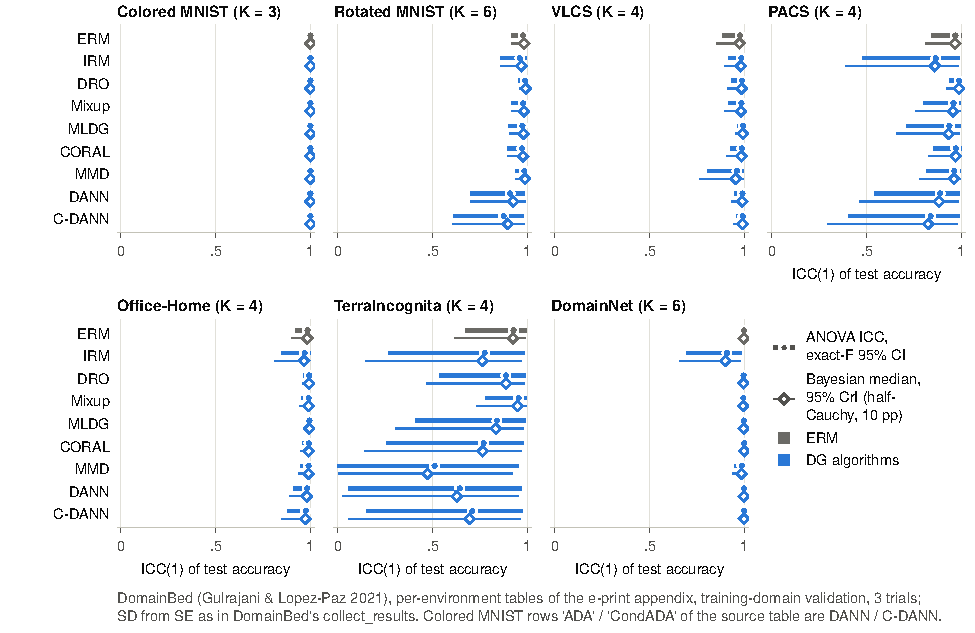
\includegraphics[width=\linewidth]{figs/fig_domainbed}
\caption{ICC(1) of test accuracy for the nine DomainBed algorithms on seven
datasets under training-domain validation (arXiv:2007.01434v1, appendix
tables; three trials per cell; SD from SE by \eqref{eq:domainbed-sd}). Filled
circles and thick bars: ANOVA estimate and exact 95\% interval
\eqref{eq:iccci}. Open diamonds and thin bars: posterior median and
equal-tailed 95\% credible interval under half-Cauchy priors (scale 10~pp).
ERM is shown in gray, the domain-generalization algorithms in blue. The
Colored MNIST rows ADA and CondADA of the source table are shown as DANN and
C-DANN.}
\label{fig:domainbed}
\end{figure}

\paragraph{Results} Table~\ref{tab:domainbed} and Fig.~\ref{fig:domainbed}
summarize the 63 fits. No dataset is run-dominated. The median ICC over the
63 fits is 0.98, and the ICC exceeds 0.8 in all 54 fits outside
TerraIncognita. Colored MNIST, DomainNet, Office-Home and VLCS are the most
strongly environment-dominated (median ICC above 0.98, median interval width
below 0.08). On Colored MNIST, every algorithm reaches 10.0--10.5\%
accuracy on the environment labeled 0.9 in the source table and
71.4--73.3\% on the other two, and the median $\hat\sigma_{\text{env}}$ is
36.1~pp against a median $\hat\sigma_{\text{run}}$ of 0.5~pp. Rotated MNIST
has the smallest spread between environments (median 1.5~pp), but its
between-trial SD is smaller still (0.3~pp). This dataset also has the most SEs
printed as 0.0 (23 of 54 cells), so rounding probably understates its run
variance and overstates its ICC. On PACS the median ICC is 0.96, but two
algorithms (IRM and C-DANN) have intervals that reach below 0.5.
TerraIncognita is the exception. Its median ICC is 0.77, its median
$\hat\sigma_{\text{run}}$ (4.0~pp) is about half its median
$\hat\sigma_{\text{env}}$ (7.5~pp), and six of its nine algorithms have
intervals with lower limits below 0.5. For MMD, the ICC is 0.51 with interval
$[0.00,0.95]$, and the $F$ test of no environment effect gives $p=0.048$.
ERM has ICC 0.93 $[0.67,0.99]$ there. With four environments, the exact interval has
3 numerator degrees of freedom, and on TerraIncognita the median width is
0.72. The Bayesian medians are close to the ANOVA estimates (median 0.76 on
TerraIncognita).

These conclusions do not depend on the SE convention. With the textbook
convention $s=\mathrm{SE}\sqrt n$, the median ICC on TerraIncognita is 0.84
and five fits, rather than eight, have lower limits below 0.5. They do depend
on the selection rule. Under leave-one-domain-out validation, 17 of the 63
fits have lower limits below 0.5, compared with 8 under training-domain
validation and 1 under test-domain (oracle) validation. One example is DANN on
Rotated MNIST, whose three trials disagree so strongly
($\hat\sigma_{\text{run}}=15.0$~pp) that its ICC is 0.00.

\paragraph{Implications for single-environment reporting} Under
training-domain validation, most of the variance of a single DomainBed run is
due to which environment is held out. On six of the seven datasets, the median over
algorithms of the ratio $\hat\sigma_{\text{env}}/\hat\sigma_{\text{run}}$
is between 4.8 and 73.5, and on TerraIncognita it is 1.9. A result on one held-out
environment therefore describes mainly that environment. On these six
datasets the spread between environments is several times the trial-to-trial
SD, so a single environment cannot stand in for the dataset. This is a reason to evaluate on
every environment, as DomainBed does, and to report the worst environment and
the spread over environments together with the mean. On TerraIncognita, the
trial-to-trial SD is a large fraction of the spread between environments, so a
single trial says little about a given environment, even though each trial
already includes a fresh hyperparameter search. Replicating trials is
necessary there, not optional. A high ICC does not show that one algorithm
beats another in every environment. That question concerns the paired
difference \eqref{M-eq:diffvar}, whose variance excludes the shared environment
effect. DomainBed's trials also differ from our seeds. A DomainBed trial
redraws the hyperparameters and the data split, whereas our seeds keep both
fixed within a fold (Section~\ref{M-sec:protocol-lodo}). The two ICCs are
therefore not on the same scale. The comparison shows only that the ICC can be
computed from what a benchmark already publishes, and that its value, and how
precisely it is known, varies with the dataset, the number of environments and
the selection rule.

\clearpage
%% Supplementary: protocol details moved from Section 3 of the main text.
\section{Additional protocol details}
\label{sup:protocol}

\subsection{Interval estimates for the variance components}
\label{sup:intervals}

With $F=\mathrm{MSB}/\mathrm{MSW}$, the exact 95\%
interval for ICC(1) \citep{searle1992variance,mcgraw1996icc} is
\begin{equation}
  \Big[\frac{F_L-1}{F_L+n_0-1},\ \frac{F_U-1}{F_U+n_0-1}\Big],\qquad
  F_L=\frac{F}{F_{0.975}(K-1,N-K)},\quad F_U=\frac{F}{F_{0.025}(K-1,N-K)},
  \label{eq:iccci}
\end{equation}
clipped to $[0,1]$ (exact for balanced data, approximate otherwise).
$\sigma_R$ receives the exact $\chi^2_{N-K}$ interval and $\sigma_D$ the
modified large-sample interval
\citep[\S3.3]{burdick1992confidence}.


\subsection{Bayesian posterior}
\label{sup:bayes}

With $K\le7$, $\hat\sigma_D$ is often at or
near zero. We therefore also report a grid posterior,
\begin{equation}
  p(\sigma_D,\sigma_R\mid \mathbf y)\ \propto\ L_R(\sigma_D,\sigma_R)\,
  \pi(\sigma_D)\,\pi(\sigma_R),
  \label{eq:posterior}
\end{equation}
where $L_R$ is the restricted likelihood ($\mu$ integrated out under a flat
prior). $\pi$ is either a half-normal prior,
$\pi(\sigma)\propto\exp\{-\sigma^2/(2A^2)\}$, or a half-Cauchy prior,
$\pi(\sigma)\propto(1+\sigma^2/A^2)^{-1}$ \citep{gelman2006prior}. Both are
independent on each SD with scale $A=0.1$ AUROC for both $\sigma_D$ and
$\sigma_R$. The half-normal places 95\% of its mass below 0.20; the half-Cauchy
has heavy tails. The posterior is computed on a $400\times300$ grid (zero plus
a geometric grid for $\sigma_D$; a geometric grid spanning the $\chi^2$ range of
the within-domain sum of squares for $\sigma_R$) with trapezoid weights. We
report posterior medians and equal-tailed 95\% credible intervals for
$\sigma_D$, $\sigma_R$ and the ICC. When REML is at the boundary or the ANOVA
estimate is truncated, we report the one-sided interval $[0,q_{0.95}]$, because
an equal-tailed interval cannot contain zero.


\subsection{Response shape}
\label{sec:protocol-response}

Whether gains are larger where ERM is weak is assessed with Oldham's
correlation $r=\operatorname{corr}(M_t-E_t,(M_t+E_t)/2)$ between the
per-domain difference and mean of the arm ($M_t$) and ERM ($E_t$)
\citep{oldham1962}. Unlike a regression of gain on baseline, it is not biased
by regression to the mean.
$r=0$ if and only if $\operatorname{Var}(M)=\operatorname{Var}(E)$, which is
tested by the Pitman--Morgan statistic $t=r\sqrt{K-2}/\sqrt{1-r^2}$ on $K-2$
degrees of freedom \citep{pitman1939,morgan1939}. We also give an exact
sign-flip permutation $p$-value over all $2^K$ swaps of $(M_t,E_t)$. The results are in Section~\ref{app:response}.

\clearpage
%% Supplementary: cohort and arm details moved from Section 5 of the main text.
\section{Additional details of the cohorts and arms}
\label{sup:setup}

\subsection{Cohorts}
\label{sup:cohorts}

\paragraph{Camelyon17-WILDS} The cohort consists of $96\times96$~px
lymph-node patches labeled tumor or normal from five hospitals
\citep{koh2021wilds,bandi2019camelyon17}. In fold $t$, the test split is a
class-balanced sample of 25,000 patches of hospital $t$, the OOD-validation
split 12,000 patches of hospital $(t-1)\bmod5$, and the training split 30,000
class-balanced patches of the other three hospitals. ID validation (12,000
patches) holds out $\max(1,\lfloor n_c/5\rfloor)$ of the $n_c$ patients of
every training hospital $c$. The patients are redrawn with a seeded generator
until the held-out set has at least 1,000 patches of each class and at most
40\% of the hospital's tumor patches, because patients contribute between 5
and 56,666 tumor patches. The 64~px cache is the central crop of the native
patch.

\paragraph{Canine cutaneous squamous cell carcinoma} Each of 44 slides was
digitized with five scanners \citep{wilm2023canine}: cs2 (Aperio ScanScope
CS2), gt450 (Aperio GT450), p1000 (3DHistech Pannoramic~1000), nz20 (Hamamatsu
NanoZoomer 2.0-HT) and nz210 (NanoZoomer S210). A domain is a scanner. The
slides are randomly split into five groups. Fold $t$ tests scanner $t$ on slide
group $t$, validates on scanner $(t-1)\bmod5$ with slide group $(t-1)\bmod5$,
and trains on the remaining three scanners and slide groups. A test domain is
therefore a new scanner and a set of slides that is absent from training under
every scanner. Four training slides (15\%) form the ID-validation split. Per
image, about 420 candidate centers are drawn, half in carcinoma polygons and
half in non-tumor tissue polygons, allocated in proportion to polygon area. Negative centers that fall inside any tumor polygon
are dropped. A patch is kept if it lies inside the image at both sizes and its
64~px crop passes an intensity filter (mean $\le225$, SD $\ge10$), and
duplicate centers are removed. Magnification is normalized to cs2: the factor
of each scanner is the median over slides of the square root of its
annotation-area ratio to cs2. Crops of 64/65/71/73/62~px (cs2, p1000, nz20,
nz210, gt450) are resized bilinearly to 64~px, and crops of
96/98/107/110/92~px to 96~px. Factors recomputed without each fold's test and
validation slides give the same crop sizes.

\paragraph{MIDOG 2021} The training set of the MIDOG~2021 challenge
\citep{aubreville2023midog} contains 150 annotated human breast cancer images
from one laboratory, 50 from each of three scanners (Hamamatsu NanoZoomer XR,
NanoZoomer S360 and Aperio ScanScope CS2). A domain is a scanner ($K=3$), and
there is no OOD-validation domain. Patches are centered on the annotated
bounding boxes of mitotic figures and non-mitotic look-alikes. ID validation
holds out 15\% of the images of every training scanner (eight per scanner),
fixed per scanner. The TIFF resolutions are 0.2263--0.2274 (XR), 0.2298 (S360)
and 0.2533 (CS2)~\textmu m/px, a difference of about 11\%. The primary cache
therefore normalizes every image to 0.25~\textmu m/px: it crops
$\mathrm{round}(P\cdot0.25/\mathrm{mpp})$~px (63--71 and 95--106~px) and
resizes bilinearly to $P\in\{64,96\}$. The un-normalized cache keeps the
magnification difference as part of the shift, as in the challenge. It is run
at the compact tier as a sensitivity analysis.

\paragraph{MIDOG++} MIDOG++ \citep{aubreville2023midogpp} provides 503
annotated 2~mm$^2$ regions of interest from seven tumor types in two species
(Table~\ref{tab:midogpp}). Its 150 breast cancer images have pixel data
identical to the MIDOG~2021 images. A domain is a tumor type ($K=7$), and
laboratory, scanner and species vary with it. Task, patch centering, scale
normalization and ID validation follow MIDOG~2021. For the 3DHistech images,
whose $x$ and $y$ resolutions differ by 0.4\%, the geometric mean is used.

\begin{table}[width=\linewidth,pos=t]
\caption{MIDOG++ domains \citep[scanners and laboratories from Table~1
of][]{aubreville2023midogpp}. Counts are the annotated mitotic figures and
non-mitotic look-alikes used in this study; resolution is from the TIFF tags.
Fold $t$ tests domain $t$ and validates on domain $(t-1)\bmod 7$.}
\label{tab:midogpp}
\footnotesize
\begin{tabular*}{\tblwidth}{@{\extracolsep{\fill}}llrrr>{\raggedright\arraybackslash}p{2.75cm}>{\raggedright\arraybackslash}p{2.2cm}l@{}}
\toprule
Tumor type & Species & Images & Mitotic & Look-alike & Scanner & Laboratory & \textmu m/px \\
\midrule
Mast cell tumor & canine & 50 & 2,327 & 1,366 & Aperio ScanScope CS2 & FU Berlin & 0.2533 \\
Lung cancer & canine & 44 & 855 & 951 & 3DHistech Pannoramic Scan II & VMU Vienna & 0.2487 \\
Lymphosarcoma & canine & 55 & 3,959 & 4,257 & 3DHistech Pannoramic Scan II & VMU Vienna & 0.2487 \\
Soft tissue sarcoma & canine & 100 & 1,286 & 2,375 & 3DHistech Pannoramic Scan II & AMC New York, VMU Vienna & 0.2487 \\
Breast cancer & human & 150 & 1,721 & 2,714 & Hamamatsu XR, S360; Aperio CS2 & UMC Utrecht & 0.2263--0.2533 \\
Melanoma & human & 49 & 1,150 & 925 & Hamamatsu XR & UMC Utrecht & 0.2263--0.2274 \\
Neuroendocrine tumor & human & 55 & 639 & 1,761 & Hamamatsu XR & UMC Utrecht & 0.2263--0.2274 \\
\midrule
Total & & 503 & 11,937 & 14,349 & & & \\
\bottomrule
\end{tabular*}
\end{table}

\paragraph{Mirror padding} MIDOG objects closer to the image border than
half a crop are cut from a reflect-padded copy of the image. The object
therefore stays centered, and its 64 and 96~px patches are concentric. At
96~px this affects 111 of 4,435 MIDOG~2021 patches and 617 of 26,286 MIDOG++
patches, at similar rates in both classes (MIDOG++: 2.43\% of positives,
2.28\% of negatives). The padding of each row is stored for a sensitivity
analysis that excludes these patches.

\paragraph{Unlabeled pools} The pool used for self-supervised pre-training
comes only from the training domains and excludes ID-validation groups, the
validation domain and the test domain. The arms that use it therefore remain
domain generalization methods and do not adapt to the test domain. On
Camelyon17 the pool consists of 40,000 patches of non-ID-validation training
patients that are not in the training split. On the other cohorts it consists
of random tissue crops (mean $<220$, SD $>12$) from non-ID-validation training
images. The crops are drawn with image-specific seeds, at most 800 per canine
image and 300 per MIDOG image, and subsampled to 40,000. MIDOG~2021 yields
only 25,200.


\subsection{Self-supervision controls and stain normalization}
\label{sup:arms}

\paragraph{Controls for self-supervision} The augmentation-only control
applies SimCLR's view augmentation to labeled batches without the contrastive
loss. It separates the effect of the augmentations from that of pre-training.
As in the SimCLR views, crop and flip parameters are drawn per batch and color
factors per image. The compute-matched control gives ERM as many images through
the encoder as SimCLR receives in pre-training and fine-tuning together.
Pre-training runs 6 epochs of $\lfloor|U|/256\rfloor$ steps on two views of 256
images, so $I_{\text{SSL}}=479{,}232$ for $|U|=40{,}000$ and 301,056 for
MIDOG~2021. SimCLR is pre-trained separately for every fold and seed, with SGD
(momentum 0.9, weight decay $10^{-4}$), a cosine schedule and projection heads
of 256--256--128 (C) or 2048--2048--128 (S). It is then fine-tuned with the ERM
recipe.

\paragraph{Stain normalization} As in common practice, Macenko's stain matrix
\citep{macenko2009} is estimated once per slide. A group is a slide imaged on
one scanner: a Camelyon17 slide, a MIDOG image, a canine slide on one of its
three scanners, or a PatchCamelyon whole-slide image. For each group, up to 256
tiles are drawn in a content-hashed order that does not depend on row order.
Their tissue pixels (optical density $\ge0.15$ in every channel; at most
200,000, subsampled with a fixed seed) are pooled. Macenko's estimator is then
applied once: the plane of the two leading eigenvectors, then the 1st and 99th
angular percentiles. The two directions are labeled hematoxylin and eosin by
matching them to the reference. Concentrations are the least-squares solution
clamped at zero, because without the clamp eosin-rich pixels received large
negative hematoxylin values on pale tiles. The group's maximal concentrations
are the per-stain 99th percentiles over its pooled pixels. Every tile is
rescaled to the reference maxima and reconstructed with the reference matrix. A
group with too little tissue keeps the reference. The reference is fitted per
fold with the same estimator on every training group: its stain matrix is the
elementwise median of the aligned group matrices, and its maxima are the median
group maxima. No labels are used. The method is transductive, however: each
test slide is normalized from its own tiles, which are the benchmark's patches
from annotated regions rather than a label-independent sample of the slide.
Section~\ref{app:macenko} reports how much the estimate depends on that tile
set, and a per-tile variant that estimates the stain matrix on every tile
separately. Our H\&E jitter perturbs RGB color; it is not an augmentation in
HED space.



\bibliographystyle{cas-model2-names}
\bibliography{main}
\end{document}
